% changelog: "1.0.0, 2024-06-04, Approvazione per RTB"

\documentclass[8pt]{article}
\usepackage[italian]{babel}
\usepackage[utf8]{inputenc}
\usepackage[letterpaper, left=1in, right=1in, bottom=0.75in, top=0.75in]{geometry}
\usepackage{amsmath}
\usepackage{subfiles}
\usepackage{lipsum}
\usepackage{csquotes}
\usepackage{amsfonts}
\usepackage[sfdefault]{plex-sans}
\usepackage{float}
\usepackage{pifont}
\usepackage{mathabx}
\usepackage[euler]{textgreek}
\usepackage{makecell}
\usepackage{tikz}
\usepackage{wrapfig}
\usepackage{siunitx}
\usepackage{amssymb} 
\usepackage{tabularx}
\usepackage{adjustbox}
\usepackage[document]{ragged2e}
\usepackage{floatflt}
\usepackage[colorlinks=true,linkcolor=nan1fyblue,urlcolor=nan1fyblue]{hyperref}
\usepackage{graphicx}
\usepackage{hyperref}
\setcounter{tocdepth}{4}
\usepackage{caption}
\usepackage{multicol}
\usepackage{tikz}
\setlength\parindent{0pt}
\captionsetup{font=footnotesize}
\usepackage{fancyhdr} 
\usepackage{graphicx}
\usepackage{capt-of}% 
\usepackage{booktabs}
\usepackage{varwidth}
\usepackage{xcolor}

\definecolor{nan1fyblue}{RGB}{23,103,162}

% -- TITOLO INTESTAZIONE -- %
\newcommand{\customtitle}{PIANO DI PROGETTO} % o ESTERNO

% -- STILE INTESTAZIONE -- %
\fancypagestyle{mystyle}{
	\fancyhf{} 
	\fancyhead[R]{
\includegraphics[height=1cm]{../../template/images/logos/NaN1fy_logo.png}} 
	\fancyhead[L]{\leftmark} 
	\renewcommand{\headrulewidth}{1pt} 
	\fancyhead[L]{\customtitle} 
	\renewcommand{\headsep}{1.3cm} 
	\fancyfoot[C]{\thepage} 
}

% -- PER LA FIRMA -- %
\newcommand{\signatureline}[1]{%
	 \par\vspace{0.5cm}
	\noindent\makebox[\linewidth][r]{\rule{0.2\textwidth}{0.5pt}\hspace{3cm}\makebox[0pt][r]{\vspace{3pt}\footnotesize #1}}%
}

% -- PER IL GLOSSARIO -- %
\newcommand{\glossterm}[1]{#1\textsuperscript{G}} % inserisci \glossterm{termine}

% -- per abilitare 4x sottosezioni es 2.1.1.1
\setcounter{secnumdepth}{4}
\newcommand{\subsubsubsection}[1]{\paragraph{#1}\mbox{}\\}

\begin{document}
\begin{titlepage}
\begin{tikzpicture}[remember picture, overlay]
      \node[anchor=south east, opacity=0.2, yshift = -4cm, xshift= 2em] at (current page.south east) {
\includegraphics[width=0.7\textwidth, trim=0cm 0cm 5cm 0cm, clip]{../../template/images/logos/Universita_Padova_transparent.png}};
		\node[anchor=north west, opacity=1, yshift = 4.2cm, xshift= 1.4cm, scale=1.6] at (current page.south west) {
\includegraphics[width=4cm]{../../template/images/logos/NaN1fy_logo.png}};
	\end{tikzpicture}
	
	\begin{minipage}[t]{0.47\textwidth}
		{\large{\textsc{Destinatari}}
			\vspace{3mm}
			\\ \large{\textsc{Prof. Tullio Vardanega}}
			\\ \large{\textsc{Prof. Riccardo Cardin}}
		}
	\end{minipage}
	\hfill
	\begin{minipage}[t]{0.47\textwidth}\raggedleft
		{\large{\textsc{Redattori}}
			\vspace{3mm}
			{\\\large{\textsc{Linda Barbiero}\\}} 
			{\large{\textsc{Guglielmo Barison\\}}}
			{\large{\textsc{Pietro Busato\\}}}
			{\large{\textsc{Veronica Tecchiati}}}
			
		}
		\vspace{8mm}
		
		{\large{\textsc{Verificatori}}
			\vspace{3mm}
			{\\\large{\textsc{Davide Donanzan}\\}}
			{\large{\textsc{Guglielmo Barison}}}
			
		}
		\vspace{4mm}\vspace{4mm}
	\end{minipage}
	\vspace{4cm}
	\begin{center}
		\begin{flushright}
			{\fontsize{30pt}{52pt}\selectfont \textbf{Piano di Progetto\\}} % o ESTERNO
		\end{flushright}
		\vspace{3cm}
	\end{center}
	\vspace{9cm}
	{\small \textsc{\href{mailto: nan1fyteam.unipd@gmail.com}{\color{black}nan1fyteam.unipd@gmail.com}}}
\end{titlepage}
\pagestyle{mystyle}
\section*{Registro delle Modifiche}
\begin{table}[ht!]	
\hypersetup{hidelinks}
	\centering
	\begin{tabular}{p{1.2cm} p{2cm} p{6cm} p{3cm} p{2cm}}
		\toprule
		\textbf{Versione}& \textbf{Data} & \textbf{Descrizione} & \textbf{Autore} & \textbf{Ruolo} \\
		\midrule 
		1.0.0 & 2024-06-04 & \textbf{Approvazione per RTB} & & \\\\
		0.11.2 & 2024-06-04 & Verifica completa e modifiche minori. & Guglielmo Barison & Verificatore \\\\
		0.11.1 & 2024-06-04 & Verifica completa e modifiche minori. & Davide Donanzan & Verificatore \\\\
		0.11.0 & 2024-05-31 & Stesura \glossterm{consuntivo} quarto periodo, correzioni minori in sezione \ref{sec:3_rtb}. & Pietro Busato & Redattore \\\\
        0.10.4 & 2024-05-21 & Correzioni minori sezione \ref{sec:3_rtb}. & Linda Barbiero & Redattore \\\\
		0.10.3 & 2024-05-21 & Aggiunte attività previste sezioni \ref{sec:1_rtb} e \ref{sec:2_rtb}, correzioni sezione \ref{sec:3_rtb}. & Veronica Tecchiati & Redattore \\\\
        0.10.2 & 2024-05-20 & Correzioni minori riguardo il primo periodo e date in sezione \ref{sec:2_rtb}. & Linda Barbiero & Redattore \\\\
		0.10.1 & 2024-05-19 & Aggiunte e correzioni sezione \ref{sec:2_rtb}. & Veronica Tecchiati & Redattore \\\\
        0.10.0 & 2024-05-17 & Stesura \glossterm{preventivo} quarto periodo, sezione \ref{sec:4_rtb}. & Pietro Busato & Redattore \\\\
		0.9.0 & 2024-05-16 & Stesura \glossterm{consuntivo} terzo periodo e correzioni minori. & Guglielmo Barison & Redattore \\\\
        0.8.0 & 2024-05-08 & Refactor struttura documento e stesura sezione \ref{sec:3_rtb}. & Guglielmo Barison & Redattore \\\\
        0.7.0 & 2024-05-03 & Stesura \glossterm{consuntivo} secondo periodo e correzioni minori. & Veronica Tecchiati & Redattore \\\\
        0.6.0 & 2024-04-30 & Stesura sezione \ref{sec:2_rtb}. & Veronica Tecchiati & Redattore \\\\
        0.5.0 & 2024-04-28 & Conclusione stesura sezione \ref{sec:rischi} & Veronica Tecchiati & Redattore \\\\
		0.4.2 & 2024-04-24 & Fix immagine diagramma \glossterm{Gantt} primo \glossterm{sprint}. & Linda Barbiero & Redattore \\\\
		0.4.1 & 2024-04-18 & Fix \glossterm{preventivo} e \glossterm{consuntivo} del primo periodo. & Linda Barbiero & Redattore \\\\
		0.4.0 & 2024-04-18 & Stesura sezione \ref{sec:1_rtb}. & Linda Barbiero & Redattore \\\\
		0.3.0 & 2024-04-17 & Inizio stesura sezione \ref{sec:rischi}. & Veronica Tecchiati & Redattore \\\\
		0.2.0 & 2024-04-16 & Stesura sezione \ref{sec:intro}. & Veronica Tecchiati & Redattore \\\\
		0.1.0 & 2024-04-12 & Stesura sezione \ref{sec:modello} e inizio sezione \ref{sec:organigramma}. & Linda Barbiero & Redattore \\\\
		0.0.0 & 2024-04-12 & Stesura del file e sezione \ref{sec:1_rtb}. & Linda Barbiero & Redattore \\
		% X.X.X & YYYY-MM-DD & Lorem ipsum dolor sit amet, consectetur adipiscing elit.  & XXXX XXXX & --- \\
		\bottomrule
		% Ruolo Redattore o Verificatore
	\end{tabular}
	\caption{Registro delle modifiche.}
	\label{table:Registro delle modifiche}
\end{table}
\newpage
{\hypersetup{hidelinks} \tableofcontents}
\clearpage
\newpage
\newpage
{\hypersetup{hidelinks} \listoffigures}
\newpage
{\hypersetup{hidelinks} \listoftables}
\newpage
\justifying
\section{Introduzione} \label{sec:intro}
\subsection{Scopo del documento}
Questo documento ha lo scopo di delineare la pianificazione e la gestione delle attività volte alla realizzazione del progetto. In particolare, saranno approfonditi temi fondamentali quali l'analisi dei rischi e la loro mitigazione, il modello di sviluppo adottato, il \glossterm{preventivo} dei costi ed il \glossterm{consuntivo}. Questo documento ha lo scopo di stabilire con chiarezza le modalità con la quale verranno eseguite
le attività dai membri del gruppo NaN1fy. In particolare verranno trattati i seguenti temi:
\begin{itemize}
\setlength\itemsep{0em}
    \item Analisi dei rischi;
    \item Organizzazione temporale delle attivit\`{a};
    \item Ripartizione dei compiti tra i componenti del gruppo;
    \item Stima dei costi e delle risorse delle varie iterazioni.
\end{itemize}
\subsection{Scopo del prodotto}
Il fine è creare una data pipeline che, partendo dalla generazione di dati da alcuni sensori simulati, possa gestire, archiviare, analizzare e visualizzare il flusso dati in tempo reale. I sensori simuleranno il campionamento di diverse caratteristiche della città in esame, come temperatura, vento, traffico e altri elementi analoghi per poi rappresentarne i dati attraverso \glossterm{dashboard} grafiche.
\subsection{Glossario}
Per garantire chiarezza nel linguaggio utilizzato nei documenti, è stato redatto un Glossario contenente le definizioni dei termini con significato specifico da disambiguare. Tali termini sono contrassegnati con una G ad apice. L'inserimento di un termine nel Glossario è considerato completo solo dopo averne fornito la definizione.


\subsection{Preventivo iniziale}
Come riportato nel preventivo presentato in fase di candidatura, viene stimato il costo totale del
progetto per un ammontare di 11 .430,00\;\texteuro. Il gruppo prevede di consegnare il
prodotto finito entro la data \textbf{2024-09-06}.

\subsection{Riferimenti}
\subsubsection{Normativi}
\begin{itemize}
\setlength\itemsep{0em}
	\item \textit{Norme di Progetto v.1.0.0};
	\item Presentazione e documentazione del capitolato d'appalto C6 - SyncCity:
	\begin{itemize}
            \setlength\itemsep{0em}
		\item \href{https://www.math.unipd.it/~tullio/IS-1/2023/Progetto/C6p.pdf}{https://www.math.unipd.it\textasciitilde{}tullio/IS-1/2023/Progetto/C6p.pdf} (Ultimo accesso: \today)
		\item \href{https://www.math.unipd.it/~tullio/IS-1/2023/Progetto/C6.pdf}{https://www.math.unipd.it/\textasciitilde{}tullio/IS-1/2023/Progetto/C6.pdf} (Ultimo accesso: \today)
	\end{itemize}
\end{itemize}

\subsubsection{Riferimenti informativi}
\begin{itemize}
\setlength\itemsep{0em}
    \item \textit{Glossario v1.0.0};
	\item Dispense T2 - Processi di ciclo di vita:
	\begin{itemize}
		\item
        \href{https://www.math.unipd.it/~tullio/IS-1/2023/Dispense/T2.pdf}{https://www.math.unipd.it/\textasciitilde{}tullio/IS-1/2023/Dispense/T2.pdf} (Ultimo accesso: \today)
	\end{itemize}
	\item Dispense T3 - Il ciclo di vita del software:
	\begin{itemize}
		\item
        \href{https://www.math.unipd.it/~tullio/IS-1/2023/Dispense/T3.pdf}{https://www.math.unipd.it/\textasciitilde{}tullio/IS-1/2023/Dispense/T3.pdf} (Ultimo accesso: \today)
	\end{itemize}
	\item Dispense T4 - Gestione di progetto:
	\begin{itemize}
		\item
        \href{https://www.math.unipd.it/~tullio/IS-1/2023/Dispense/T4.pdf}{https://www.math.unipd.it/\textasciitilde{}tullio/IS-1/2023/Dispense/T4.pdf} (Ultimo accesso: \today)
	\end{itemize}
\item Dispense T5 - Analisi dei requisiti:
	\begin{itemize}
		\item
        \href{https://www.math.unipd.it/~tullio/IS-1/2023/Dispense/T5.pdf}{https://www.math.unipd.it/\textasciitilde{}tullio/IS-1/2023/Dispense/T5.pdf} (Ultimo accesso: \today)
	\end{itemize}
    \end{itemize}

\clearpage
\section{Analisi dei Rischi} \label{sec:rischi}
Sono molteplici gli imprevisti che si possono manifestare durante la realizzazione di un progetto. Se non affrontate correttamente, le problematiche riscontrate possono impattare negativamente sullo svolgimento delle attività, causando un aumento dei costi, ritardi nel processo di sviluppo e una diminuzione della \glossterm{qualità} del prodotto. Pertanto, si rivela essenziale condurre un'analisi approfondita dei rischi che possono insorgere, con l'obiettivo di prevenirli o quantomeno attenuarne gli effetti. \\
Il \glossterm{processo} di mitigazione si compone quindi delle seguenti fasi: 
\begin{itemize}
\setlength\itemsep{0em}
    \item \textbf{Identificazione:} individuazione della minaccia, riconoscendone origine e contesto d'insorgenza;
    \item \textbf{Valutazione:} stima della probabilità di occorrenza e assegnazione di un grado di pericolosità indicativo del potenziale impatto sul progetto;
    \item \textbf{Mitigazione:} adozione di strategie di prevenzione e contrasto delle possibili conseguenze negative derivanti da una situazione avversa.
\end{itemize}
Per garantire uno svolgimento efficiente del progetto è necessario compiere un monitoraggio periodico delle attività, in modo da riconoscere eventuali nuovi rischi o aggiornare un processo di mitigazione precedentemente definito. \\ Di seguito sono elencati i rischi individuati, suddivisi per contesto d'insorgenza.

\subsection{Rischi tecnologici}
\subsubsection{RT-1 Inesperienza}
La scarsa conoscenza delle tecnologie richieste per la realizzazione del prodotto determina la necessità di formazione preliminare alle fasi di progettazione e sviluppo, con conseguenti possibili ritardi.
\begin{itemize}
\setlength\itemsep{0em}
    \item \textbf{Identificazione:} ciascun membro del gruppo ha notificato il proprio grado di conoscenza delle tecnologie richieste dal \glossterm{capitolato} agli altri componenti e alla \glossterm{Proponente}. In questo modo è stato più semplice desumere i punti di forza del fornitore e gli argomenti che invece avrebbero necessitato di maggiori approfondimenti;
    \item \textbf{Valutazione:} pericolosità: alta; probabilità: alta;
    \item \textbf{Mitigazione:} la Proponente si è resa disponibile ad assistere il team nell'apprendimento di alcune tecnologie, grazie ad incontri dedicati e al sostegno di una figura competente in grado di fornire supporto tecnico. In aggiunta, il gruppo organizzerà dei \textit{workshop} interni, oltre a prevedere il lavoro di coppia per lo svolgimento di determinati compiti. L'aiuto reciproco e la condivisione delle conoscenze rendono infatti più efficiente il \glossterm{processo} di formazione e aiutano a rafforzare lo spirito di squadra.
\end{itemize}

\subsubsection{RT-2 Produzione di codice incomprensibile}
La partecipazione alla stesura del codice sorgente da parte di diversi membri del gruppo, ciascuno con il proprio grado di esperienza e stile di programmazione, può portare alla produzione di codice difficilmente leggibile, il quale può generare fraintendimenti ed essere sintomo di scarsa \glossterm{qualità} del prodotto. 
\begin{itemize}
\setlength\itemsep{0em}
    \item \textbf{Identificazione:} questa problematica si manifesta quando risulta difficoltoso interpretare il codice scritto da altri componenti, al punto da causare un aumento di discussioni interne;
    \item \textbf{Valutazione:} pericolosità: media; probabilità: media;
    \item \textbf{Mitigazione:} saranno adottate delle convenzioni di codifica con l'obiettivo di rendere omogeneo e maggiormente manutenibile il codice prodotto. Esso sarà inoltre corredato dell'adeguata documentazione e soggetto a revisioni continue.
\end{itemize}

\subsubsection{RT-3 Perdita delle informazioni}
I file contenenti la documentazione ed il codice sorgente potrebbero essere soggetti a danneggiamento a causa di errori umani o malfunzionamenti hardware, inficiando così il normale proseguimento del lavoro.
\begin{itemize}
\setlength\itemsep{0em}
    \item \textbf{Identificazione:} il rischio si concretizza nel momento in cui si verifica un guasto, si effettuano modifiche indesiderate o si eliminano accidentalmente i file del progetto;
    \item \textbf{Valutazione:} pericolosità: alta; probabilità: bassa;
    \item \textbf{Mitigazione:} i file sono mantenuti in una \glossterm{repository} remota, in modo garantire a tutti i membri del gruppo la possibilità di accedervi agevolmente e preservarli da eventuali malfunzionamenti dei singoli dispositivi. Inoltre, viene adottato un sistema di \glossterm{versionamento} per consentire il recupero di versioni precedenti, proteggendo così i documenti da alterazioni sgradite dovute ad errori umani. 
\end{itemize}

\subsection{Rischi di comunicazione}
\subsubsection{RC-1 Scarsa comunicazione interna}
Una comunicazione interna inefficace può causare fraintendimenti e disorganizzazione, generando tensione e sconforto tra i componenti del gruppo. Questa problematica impatta ovviamente anche sull'adeguato proseguimento delle attività, che potrebbe infatti subire significativi ritardi.
\begin{itemize}
\setlength\itemsep{0em}
    \item \textbf{Identificazione:} l'eccessiva durata delle riunioni interne, la reiterazione di questioni già affrontate in precedenza e incomprensioni frequenti suggeriscono l'occorrenza di questa complicazione;
    \item \textbf{Valutazione:} pericolosità: alta; probabilità: bassa;
    \item \textbf{Mitigazione:} la prevenzione di questo rischio è messa in atto grazie all'utilizzo di diversi canali di comunicazione, all'organizzazione di incontri periodici, alla definizione anticipata dell'ordine del giorno delle riunioni e alla produzione di documentazione adeguata per tenere traccia delle decisioni prese e delle discussioni affrontate.
\end{itemize}

\subsubsection{RC-2 Scarsa comunicazione con la \glossterm{Proponente}}
Comunicare con la Proponente in modo sporadico e disorganizzato potrebbe compromettere significativamente la \glossterm{qualità} del prodotto realizzato. Inoltre, l'azienda ricopre il ruolo di mentore del gruppo, dunque svolgere le attività previste senza un adeguato supporto può provocare caos e smarrimento.
\begin{itemize}
\setlength\itemsep{0em}
    \item \textbf{Identificazione:} sintomi di questa problematica sono la riproposizione dei medesimi quesiti alla proponente da parte del gruppo fornitore e incomprensioni riguardanti le aspettative sul prodotto da realizzare;
    \item \textbf{Valutazione:} pericolosità: alta; probabilità: bassa;
    \item \textbf{Mitigazione:} si terranno incontri periodici per verificare lo stato di avanzamento del lavoro (\glossterm{SAL}). La proponente ha inoltre predisposto un canale di messaggistica istantanea, in aggiunta alla comunicazione via mail, per chiarire i dubbi che insorgono durante lo svolgimento delle attività assegnate.
\end{itemize}

\subsubsection{RC-3 Conflitti interni}
Durante lo svolgimento del progetto potrebbero sorgere dei contrasti dovuti alla diversità di opinioni, con il rischio di influire negativamente sulla capacità decisionale del gruppo, rallentando così il proseguimento delle attività.
\begin{itemize}
\setlength\itemsep{0em}
    \item \textbf{Identificazione:} il problema si manifesta quando, osservando le dinamiche interne al gruppo, si riconoscono tensioni tra i membri, si verificano discussioni ripetute e vi è una diffusa diffidenza;
    \item \textbf{Valutazione:} pericolosità: media; probabilità: bassa;
    \item \textbf{Mitigazione:} a ciascun membro del team viene offerto lo spazio sufficiente per esprimere le proprie idee ed avanzare nuove proposte. Ciascuna iniziativa diverrà poi oggetto di discussione interna, la quale si concluderà con una votazione. Affinché il confronto avvenga sempre in modo rispettoso e sia garantito il raggiungimento di una soluzione concreta in tempi ragionevoli, il responsabile assumerà il ruolo di mediatore, supervisionando i dibattiti con l'obiettivo di trovare un accordo soddisfacente.
\end{itemize}

\subsubsection{RC-4 Confusione nella rotazione dei ruoli}
La mancanza di chiarezza sui ruoli ricoperti e sulle responsabilità assunte da ciascuna componente del gruppo può impattare negativamente sull'organizzazione delle attività e generare conflitti interni.
\begin{itemize}
\setlength\itemsep{0em}
    \item \textbf{Identificazione:} si riscontrano frequentemente perplessità sul lavoro svolto sino a quel momento, dovute ad una pianificazione disordinata oppure ad una comunicazione scarsa o ambigua;
    \item \textbf{Valutazione:} pericolosità: media; probabilità: media;
    \item \textbf{Mitigazione:} è necessario definire chiaramente le responsabilità di ciascuno ancor prima di cimentarsi nello svolgimento delle attività. Successivamente, è indispensabile che ogni membro comprenda come ricoprire il proprio ruolo nella maniera più consona. Pertanto, la persona che ha svolto la medesima funzione nello \glossterm{Sprint} precedente condividerà le conoscenze acquisite con il suo successore, al fine di facilitare l'apprendimento degli incarichi assegnati.
\end{itemize}

\subsection{Rischi di pianificazione}
\subsubsection{RP-1 Stima errata delle tempistiche di progetto}
Al momento del calcolo del \glossterm{preventivo} iniziale il gruppo non ha un livello di esperienza tale da consentire una stima accurata del tempo necessario al raggiungimento delle \glossterm{milestone} del progetto. La previsione potrebbe quindi rivelarsi inesatta, portando, nel peggiore dei casi, ad un considerevole ritardo nello svolgimento del progetto.
\begin{itemize}
\setlength\itemsep{0em}
    \item \textbf{Identificazione:} questa complicazione si verifica quando risulta evidente che la data prevista per il raggiungimento di una milestone differisce significativamente dalla data di effettivo completamento delle attività relative alla suddetta milestone;
    \item \textbf{Valutazione:} pericolosità: alta; probabilità: media;
    \item \textbf{Mitigazione:} aggiornamenti frequenti sull'avanzamento del progetto permettono di adottare una pianificazione flessibile. Le attività sono quindi di volta in volta pianificate con l'obiettivo di rispettare i tempi stabiliti.
\end{itemize}

\subsubsection{RP-2 Stima errata dei costi di progetto}
Al momento del calcolo del preventivo iniziale il gruppo non ha un livello di esperienza tale da consentire una stima accurata e realistica dei costi, che potrebbero quindi subire variazioni impreviste.
\begin{itemize}
\setlength\itemsep{0em}
    \item \textbf{Identificazione:} una manifestazione lampante di questa problematica è un eccessivo divario tra preventivo e \glossterm{consuntivo}, riscontrabile grazie ad un confronto con quanto riportato nel \textit{Piano di Progetto};
    \item \textbf{Valutazione:} pericolosità: alta; probabilità: media;
    \item \textbf{Mitigazione:} il calcolo del preventivo ad ogni \glossterm{Sprint} e la corrispondente rendicontazione del consuntivo di periodo permettono di maturare accuratezza nelle previsioni e monitorare i costi effettivi. La proponente viene informata periodicamente di eventuali variazioni.
\end{itemize}

\subsubsection{RP-3 Stima errata del tempo di completamento di un'attività}
La sottostima o la sovrastima del tempo necessario per lo svolgimento di un incarico possono portare rispettivamente allo slittamento delle attività già pianificate o all'attesa superflua per il proseguimento del lavoro. Entrambe gli errori di valutazione possono provocare ritardi nello sviluppo.
\begin{itemize}
\setlength\itemsep{0em}
    \item \textbf{Identificazione:} questo rischio si concretizza quando, durante le retrospettive sul lavoro svolto, si notano discrepanze tra l'intervallo temporale preventivato per lo svolgimento di un singolo compito e le ore effettivamente impiegate;
    \item \textbf{Valutazione:} pericolosità: media; probabilità: alta;
    \item \textbf{Mitigazione:} aggiornamenti frequenti sull'avanzamento del progetto permettono di adottare una pianificazione flessibile. Il Responsabile può quindi assegnare maggiori risorse ad attività che si rivelano essere più onerose del previsto e viceversa. In aggiunta, la ripetizione in ogni Sprint dell'attività di valutazione delle tempistiche consente di sviluppare maggiore precisione, producendo man mano stime sempre più realistiche.
\end{itemize}

\subsubsection{RP-4 Variazione requisiti di progetto}
La possibilità i requisiti cambino in corso d'opera può comportare la necessità di revisione della pianificazione iniziale e l'adeguamento del lavoro svolto alle nuove richieste, causando ritardi e aumenti dei costi.
\begin{itemize}
\setlength\itemsep{0em}
    \item \textbf{Identificazione:} la \glossterm{Proponente} comunica al fornitore nuove esigenze, differenti da quanto riferito in precedenza. Ciò si traduce in modifiche da apportare a quanto già prodotto o aggiunte non previste;
    \item \textbf{Valutazione:} pericolosità: alta; probabilità: bassa;
    \item \textbf{Mitigazione:} il team viene aggiornato regolarmente dalla Proponente grazie a comunicazioni chiare ed opportunamente frequenti. L'azienda ha modo di constatare la conformità del prodotto alle aspettative descritte mediante incontri periodici di revisione dell'operato (\glossterm{SAL}).
\end{itemize}

\subsubsection{RP-5 Impegni personali ed accademici}
Durante le settimane predisposte allo svolgimento del progetto i componenti del gruppo potrebbero imbattersi in alcuni impedimenti esterni indeclinabili, quali esami universitari, problemi di salute o altre tipologie di incombenze. 
Ciò può indurre a diminuire il quantitativo di ore dedicate all'esecuzione delle attività previste, con conseguenti rallentamenti.
\begin{itemize}
\setlength\itemsep{0em}
    \item \textbf{Identificazione:} ciascuno notifica al team i propri impegni nel momento in cui viene a conoscenza della loro occorrenza;
    \item \textbf{Valutazione:} pericolosità: media; probabilità: bassa;
    \item \textbf{Mitigazione:} per ovviare alle conseguenze negative di questo rischio è utile effettuare una pianificazione delle attività che tenga in considerazione gli impegni inevitabili di ognuno. Pertanto, se dovesse rivelarsi necessario, le ore di lavoro assegnate durante i periodi di disponibilità limitata possono essere ridotte, ricollocando di conseguenza le scadenze prefissate. 
\end{itemize}

\subsection{Tabella riassuntiva}
Segue una sintesi dei rischi sopracitati, riportandone in particolare il grado di pericolosità e la probabilità di occorrenza.

\begin{table}[ht!]
    \centering
    \renewcommand{\arraystretch}{1.25}
    \begin{tabular}{cccc}
        \toprule
        \textbf{Codice} & \textbf{Rischio} & \textbf{Pericolosità} & \textbf{Probabilità} \\ \midrule
        RT-1 & Inesperienza & Alta & Alta \\ 
        RT-2 & Produzione di codice incomprensibile & Media & Media \\ 
        RT-3 & Perdita delle informazioni & Alta & Bassa \\ 
        RC-1 & Scarsa comunicazione interna & Alta & Bassa \\ 
        RC-2 & Scarsa comunicazione con la \glossterm{Proponente} & Alta & Bassa \\ 
        RC-3 & Conflitti interni & Media & Bassa \\ 
        RC-4 & Confusione nella rotazione dei ruoli & Media & Media \\ 
        RP-1 & Stima errata delle tempistiche di progetto & Alta & Media \\ 
        RP-2 & Stima errata dei costi di progetto & Alta & Media \\ 
        RP-3 & Stima errata del tempo di completamento di un'attività & Media & Alta \\ 
        RP-4 & Variazione requisiti di progetto & Alta & Bassa \\ 
        RP-5 & Impegni personali ed accademici & Media & Bassa \\ 
        \bottomrule
    \end{tabular}
    \caption{Tabella riassuntiva dei rischi.}
    \label{table:Tabella riassuntiva dei rischi}
\end{table}
\newpage

\section{Modello di Sviluppo} \label{sec:modello}
\subsection{Modello Agile}
Un approccio metodologico agile fornisce un insieme di caratteristiche che lo rendono particolarmente idoneo per gestire le tempistiche limitate di rilascio, garantendo comunque un progetto di \glossterm{qualità} buona.
Questa metodologia prevede la realizzazione di molteplici rilasci successivi, ciascuno dei quali porta con sé un incremento delle \glossterm{funzionalità}. Adottando tale approccio, diventa essenziale identificare e classificare i requisiti in modo da definire un ordine di priorità nello sviluppo, consentendo di ottenere, dopo ogni incremento, un prodotto stabile e funzionante, seppur incompleto. Per garantire la stabilità del prodotto sin dalle prime fasi, è cruciale che i primi incrementi soddisfino i requisiti più significativi, mentre quelli di minore importanza saranno integrati in un secondo momento, permettendo loro di stabilizzarsi gradualmente nel contesto del prodotto.
\\\\
I vantaggi da evidenziare sono i seguenti:
\begin{itemize}
\setlength\itemsep{0em}
\item
\textbf{Iterazioni rapide:} \glossterm{Sprint} brevi e frequenti permettono di ottenere risultati tangibili in tempi rapidi e di adattare il piano di sviluppo in base ai feedback e alle esigenze emergenti;
\item
\textbf{Flessibilità e adattabilità:} si portanno apportare modifiche al prodotto anche in corso d'opera senza dover ripensare completamente il \textit{Piano di Progetto};
\item
\textbf{Coinvolgimento del cliente/\glossterm{Proponente}:} permette il coinvolgimento col Proponente continuo durante tutto il ciclo di sviluppo, così da avere feedback tempestivi e garantire che il prodotto finale soddisfi effettivamente le esigenze;
\item
\textbf{Focus sulla qualità:} la pratica di sviluppo incrementale, al testing continuo e al coinvolgimento degli \glossterm{stakeholder} consente comunque di mantere alta la qualità del software;
\item
\textbf{Comunicazione e collaborazione:} i membri del team rimangono allineati sugli obiettivi e sulle priorità del progetto, riducendo i rischi di fraintendimenti e conflitti.
\end{itemize}

\newpage
\section{Scadenze}
I periodi vengono suddivisi in 3 grandi insiemi corrispondenti alle revisioni di avanzamento del progetto:
\begin{itemize}
\setlength\itemsep{0em}
\item \textbf{\glossterm{RTB} (Requirements and Technology Baseline):} 2024-06-07;
\item \textbf{\glossterm{PB} (Product Baseline):} 2024-09-06.
\end{itemize}

\section{\glossterm{RTB}}
\textbf{Inizio:} 2024-04-01\\
\textbf{Fine prevista:} 2024-06-07
\subsection{Primo periodo} \label{sec:1_rtb}
\textbf{Inizio:} 2024-04-01\\
\textbf{Fine prevista:} 2024-04-19
\subsubsection{Pianificazione}
Nella fase iniziale, assume prioritaria importanza la discussione di tutte le regole precedentemente adottate e implementate nel corso del progetto, ma che non sono ancora state formalizzate mediante documentazione. Questo \glossterm{processo} mira a produrre un documento scritto accessibile a tutti i membri del team, al fine di dissipare eventuali ambiguità riguardo l'esecuzione delle attività e l'utilizzo delle risorse.
\\
Inoltre, durante questa fase, è cruciale identificare tutti i potenziali rischi che potrebbero ostacolare il progresso del progetto, al fine di prevenirli e non essere colti impreparati. Un'altra priorità consiste nell'avviare la pianificazione delle prime attività e delle relative \glossterm{milestone}, al fine di organizzare le risorse disponibili e fornire una stima preventiva dei tempi e dei costi. \\
Le attività previste per il primo periodo sono dunque le seguenti:
\begin{itemize}
\setlength{\itemsep}{0em}
    \item Avvio della stesura dei documenti \textit{Piano di Progetto}, \textit{Glossario}, \textit{Norme di Progetto}, \textit{Piano di Qualifica} e \textit{Analisi dei Requisiti};
    \item Realizzazione di un generatore dati in grado di simulare un sensore di temperatura;
    \item Predisposizione di un \glossterm{container} \glossterm{Docker} con all'interno un'installazione della tecnologia \glossterm{Kafka}.
\end{itemize}

\subsubsection{Rischi attesi}
I rischi che ci aspettiamo di correre in questo periodo sono i seguenti: 
\begin{itemize}
\setlength{\itemsep}{0em}
\item \textbf{RT-1}: Inesperienza;
\item \textbf{RP-1}: Stima errata delle tempistiche di progetto;
\item \textbf{RP-2}: Stima errata dei costi di progetto;
\item \textbf{RC-1}: Scarsa comunicazione interna;
\item \textbf{RC-3}: Conflitti interni.
\end{itemize}
Questo perchè, essendo all'inizio del progetto, siamo ancora incerti su molti aspetti di
quest'ultimo, ci stiamo attualmente organizzando e dobbiamo apprendere ancora molto. Dunque la
probabilità di incorrere in qualche problema tra quelli riportati è abbastanza elevata.
\newpage
\subsubsection{\glossterm{Preventivo}}
\subsubsubsection{Preventivo orario}
\begin{table}[ht!]
	\centering
	\begin{tabular}{p{4cm} p{1cm} p{1cm} p{1cm} p{1cm} p{1cm} p{1cm} p{3cm}}
		\toprule
        \textbf{Membro} & \multicolumn{6}{c}{\textbf{Ruoli}} & \textbf{Totale (persona)}\\
		& \textbf{AM} & \textbf{RE} & \textbf{PT} & \textbf{AN} & \textbf{PR} & \textbf{VE}\\
		\midrule
        Linda Barbiero          & -     & 3     & -     & 2     & -     & 1     & 6 \\
        Guglielmo Barison       & 3     & -     & 1     & 1     & 2,5   & 1     & 8,5\\
        Pietro Busato           & 3     & -     & 1     & 1     & 2,5   & 1     & 8,5 \\
        Davide Donanzan         & 3     & -     & -     & 3     & -     & 1,5   & 7,5 \\
        Oscar Konieczny         & 3     & -     & -     & 1     & -     & 1     & 5 \\
        Veronica Tecchiati      & 3     & -     & -     & 4     & -     & 1     & 8 \\
        \bottomrule
        \textbf{Totale (ruolo)} & 15     & 3     & 2     & 12   & 5     & 6,5   & 43,5 \\
	\end{tabular}
	\caption{Distribuzione delle ore del primo Sprint secondo ruolo e membro.}
	\label{table:Distribuzione delle ore del primo Sprint secondo ruolo e membro}
\end{table}
\begin{figure}[ht!]
    \centering
    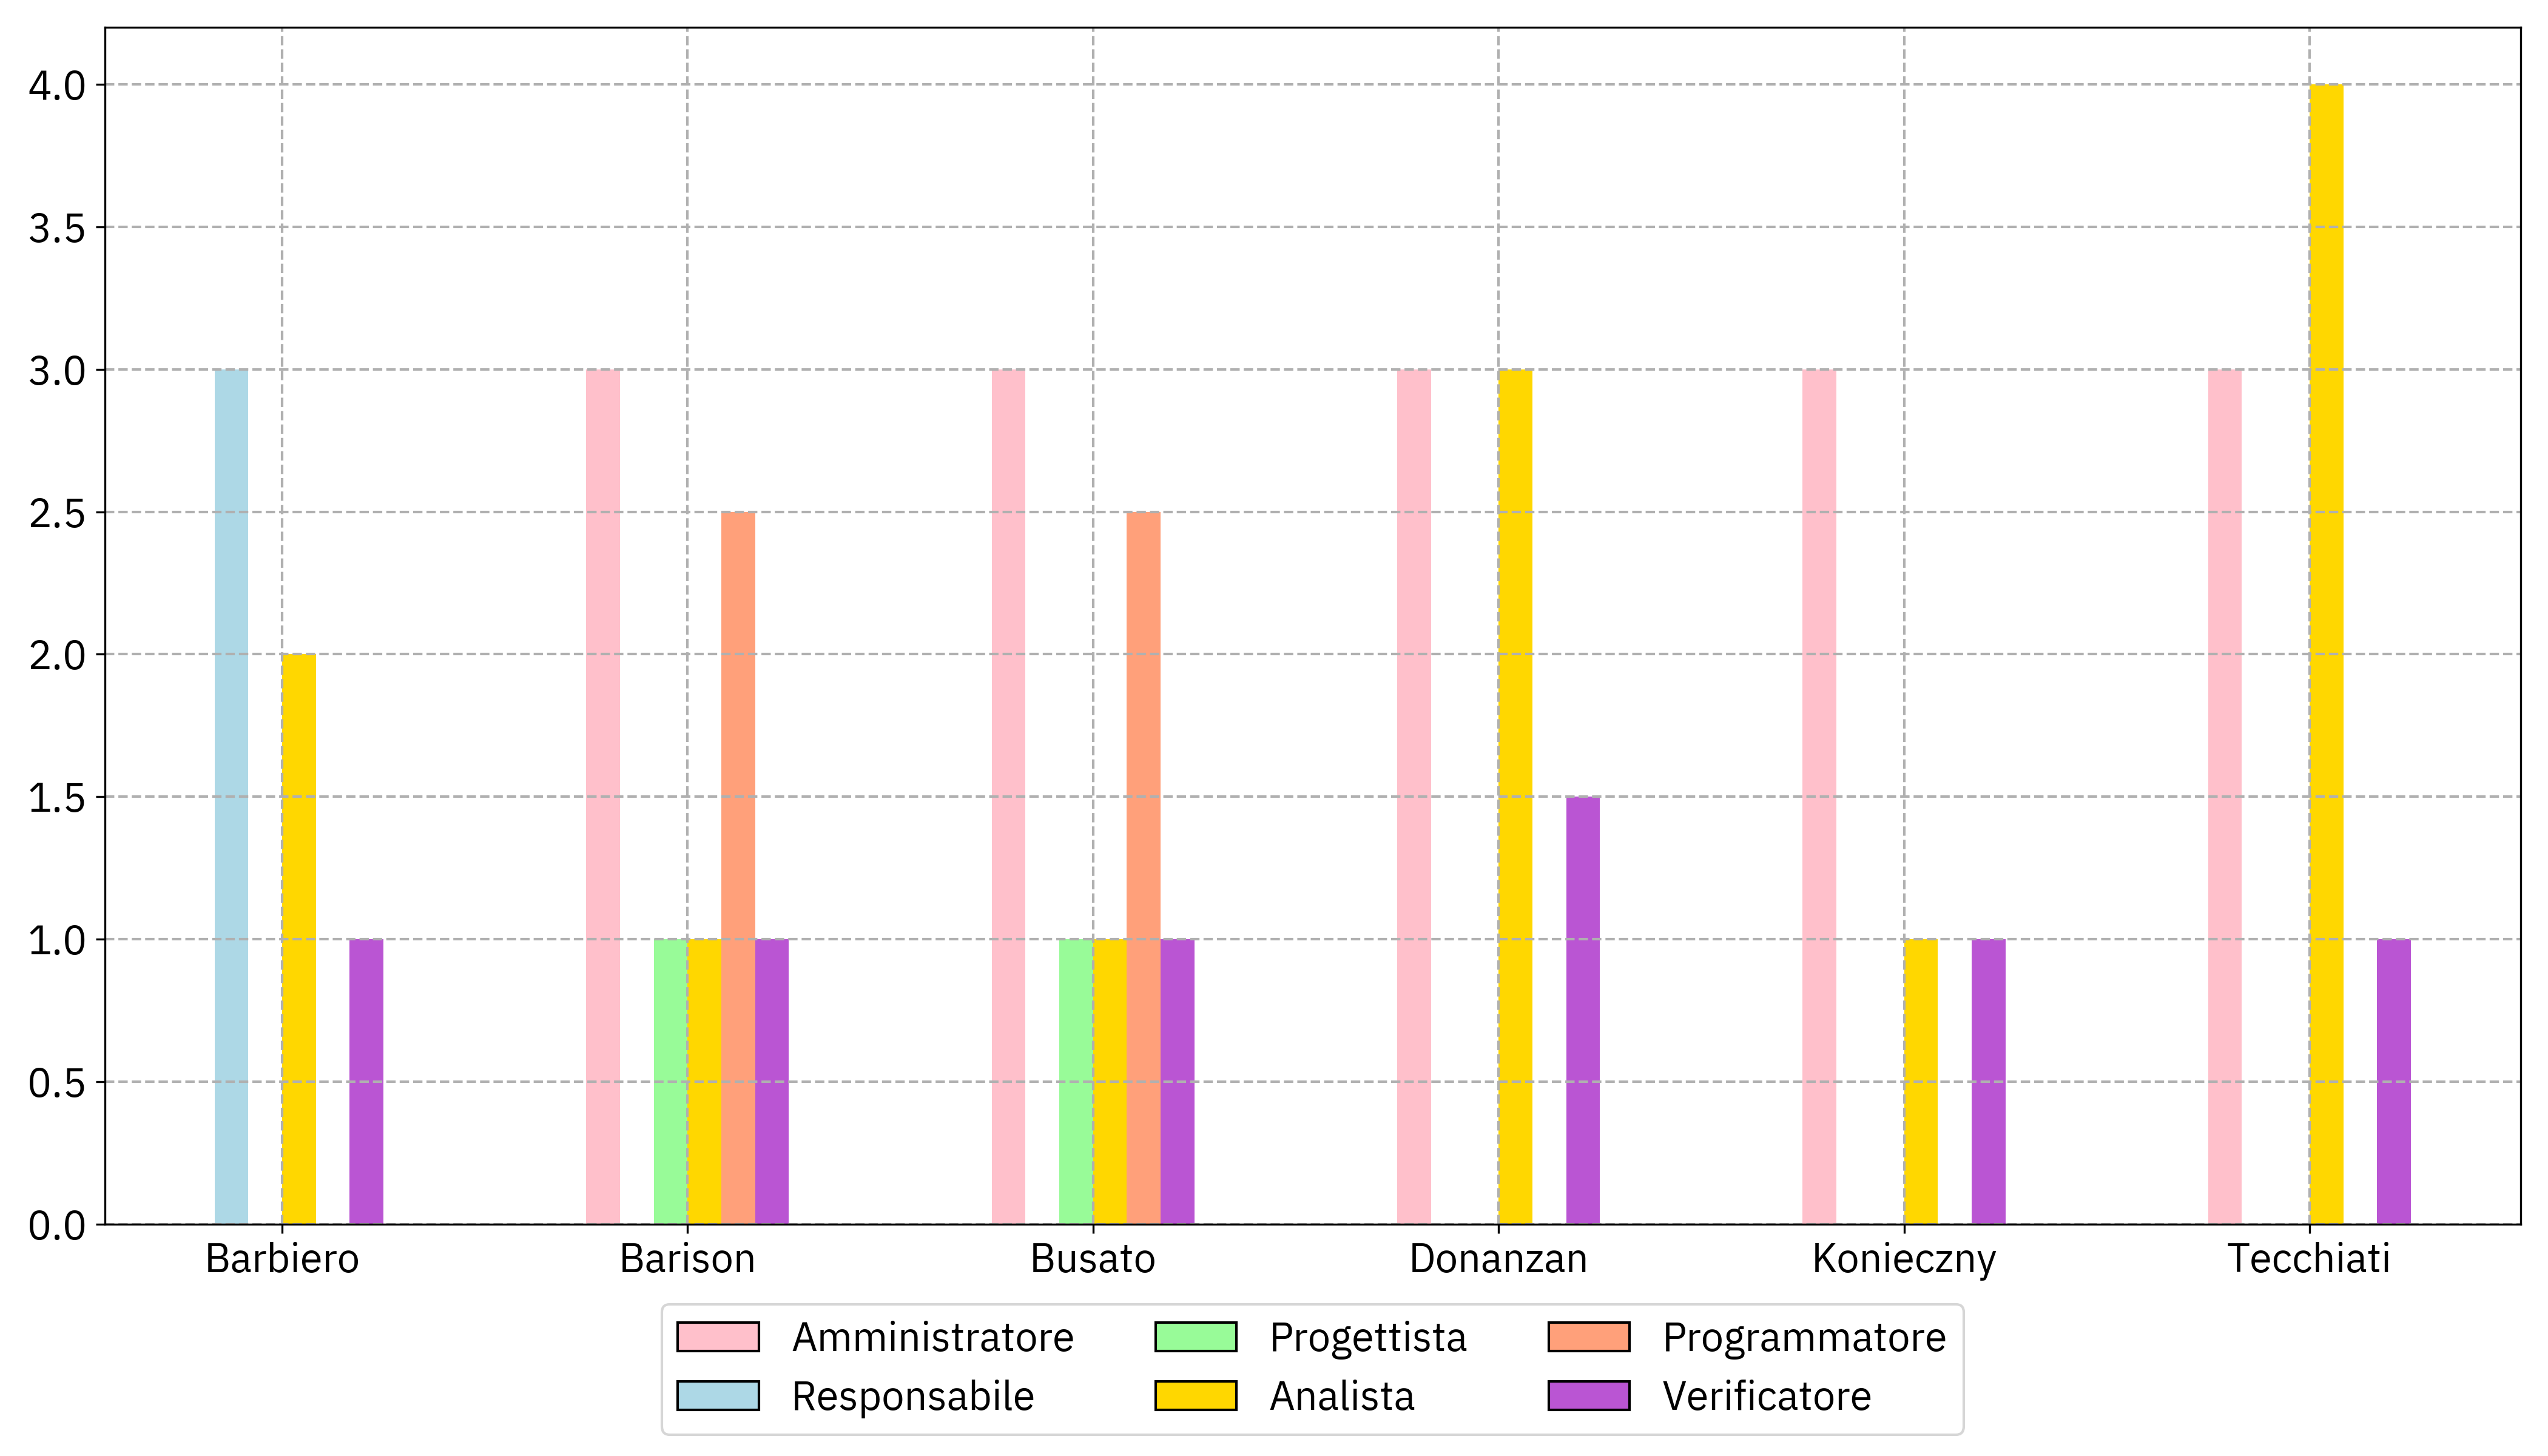
\includegraphics[width=15cm]{./images_pdp/istogramma_periodo_1.png}
    \caption{Visualizzazione dell'impegno temporale di ciascun membro nei rispettivi ruoli assegnati
    nel primo Sprint.}
    \label{figure:Visualizzazione dell'impegno temporale di ciascun membro nei rispettivi ruoli
    assegnati nel primo Sprint}
\end{figure}
\subsubsubsection{Preventivo economico}
\begin{table}[ht!]
	\centering
	\begin{tabular}{p{4cm} p{1cm} p{2cm}}
        \toprule
        \textbf{Ruolo} & \textbf{Ore} & \textbf{Costo (€)} \\
        \midrule
        Amministratore & 15 & 450 \\
        Responsabile & 3 & 60 \\
        Progettista & 2 & 50 \\
        Analista & 12 & 300 \\
        Programmatore & 5 & 75 \\
        Verificatore & 6,5 & 97,5 \\
        \bottomrule
        \textbf{Totale} & 43,5 & 1032,5
    \end{tabular}
    \caption{\glossterm{Preventivo} dei costi del primo Sprint secondo ruolo.}
	\label{table:Preventivo dei costi del primo Sprint secondo ruolo}
\end{table}
\subsubsection{\glossterm{Consuntivo}}
\subsubsubsection{Consuntivo orario}
\begin{table}[ht!]
	\centering
	\begin{tabular}{p{3cm} p{1.5cm} p{1.5cm} p{1.5cm} p{1.5cm} p{1.5cm} p{1.5cm} p{1cm}}
		\toprule
        \textbf{Membro} & \multicolumn{5}{c}{\textbf{Ruoli}} & \multicolumn{2}{r}{\textbf{Totale
        (pers.)}}\\
		& \textbf{AM} & \textbf{RE} & \textbf{PT} & \textbf{AN} & \textbf{PR} & \textbf{VE}\\
		\midrule
        Linda Barbiero          & -     & 3     & -     & 2     & 0     & 0.5 \textcolor{teal}{(-0,5)}   & 5,5 \\
        Guglielmo Barison       & 3     & -     & 1     & 1     & 2,5   & 1     & 8,5\\
        Pietro Busato           & 3     & -     & 1     & 1     & 2,5   & 1     & 8,5 \\
        Davide Donanzan         & 3     & -     & -     & 3     & -     & 2 \textcolor{teal}{(-0,5)}     & 8 \\
        Oscar Konieczny         & 3,5 \textcolor{teal}{(-0,5)}  & -     & -     & 1     & -     & 1     & 5,5 \\
        Veronica Tecchiati      & 3,5 \textcolor{teal}{(-0,5)}  & -     & -     & 5 \textcolor{teal}{(-1)}    & -     & 1     & 9,5 \\
        \bottomrule
        \textbf{Totale (ruolo)} & 16    & 3     & 2     & 13   & 5     & 6,5   & 45,5 \\
	\end{tabular}
	\caption{Distribuzione delle ore del primo Sprint secondo ruolo e membro.}
	\label{table:Distribuzione delle ore consuntive del primo Sprint secondo ruolo e membro}
\end{table}
\begin{table}[ht!]
	\centering
	\begin{tabular}{p{4cm} p{1cm} p{1cm} p{1cm} p{1cm} p{1cm} p{1cm} p{3cm}}
		\toprule
        \textbf{Membro} & \multicolumn{6}{c}{\textbf{Ruoli}} & \textbf{Totale (persona)}\\
		& \textbf{AM} & \textbf{RE} & \textbf{PT} & \textbf{AN} & \textbf{PR} & \textbf{VE}\\
		\midrule
        Linda Barbiero          & 7     & 5     & 20     & 11   & 24     & 22,5   & 89,5 \\
        Guglielmo Barison       & 4     & 9     & 19     & 11   & 21,5   & 22     & 86,5\\
        Pietro Busato           & 6     & 8     & 19     & 11   & 20,5   & 22     & 86,5 \\
        Davide Donanzan         & 6     & 8     & 20     & 9    & 23     & 21     & 87 \\
        Oscar Konieczny         & 4,5   & 7     & 20     & 11   & 24     & 23     & 89,5 \\
        Veronica Tecchiati      & 4,5   & 8     & 20     & 6    & 25     & 22     & 85,5 \\
        \bottomrule
        \textbf{Totale (ruolo)} & 32    & 45    & 118    & 59   & 138     & 132,5 & 524,5 \\
	\end{tabular}
	\caption{Ore rimaste dopo il primo Sprint secondo ruolo e membro.}
	\label{table:Ore rimaste dopo il primo Sprint secondo ruolo e membro}
\end{table}
\subsubsubsection{Consuntivo economico}
\begin{table}[ht!]
	\centering
	\begin{tabular}{p{4cm} p{2cm} p{2cm}}
        \toprule
        \textbf{Ruolo} & \textbf{Ore} & \textbf{Costo (€)} \\
        \midrule
        Amministratore & 16 \textcolor{red}{(+1)} & 480 \textcolor{red}{(+30)} \\
        Responsabile & 3 & 60 \\
        Progettista & 2 & 50 \\
        Analista & 13 \textcolor{teal}{(-1)} & 325 \textcolor{teal}{(-25)} \\
        Programmatore & 5 & 75 \\
        Verificatore & 6,5 & 97,5 \\
        \bottomrule
        \textbf{Totale} & 45,5 & 1087,5
    \end{tabular}
    \caption{\glossterm{Preventivo} a finire dei costi del primo Sprint secondo ruolo.}
	\label{table:Preventivo a finire dei costi del primo Sprint secondo ruolo}
\end{table}
\subsubsubsection{Rischi occorsi, impatto e loro mitigazione}
In questo periodo sono sorte alcune delle complicazioni previste, in particolare quelle relative alla pianificazione. Alcune attività hanno subito lievi ritardi, il che comporta la necessità di proseguirne l'esecuzione durante lo \glossterm{Sprint} successivo. Inoltre, al termine dello Sprint è stata riscontrata una discrepanza tra i costi preventivati e quelli effettivi, sebbene la differenza sia minima. A fronte di ciò, risulta al gruppo evidente quanto sia importante effettuare una pianificazione che sia fattibile in base alla mole di lavoro, promettendosi una migliore attenzione sul lato della pianificazione dei futuri Sprint.
\subsubsection{Retrospettiva}
Dal consuntivo è risultata una leggera discrepanza con il preventivo del periodo. Sono servite più ore da Amministratore e da Analista del preventivato.
Ciò ha comportato una spesa maggiore di 55\;\texteuro, per un complessivo di 1.\,087,5\;\texteuro\
rispetto ai 1\,.032,5\;\texteuro\ previsti.
In conclusione, il budget rimanente è di 10\,.342,5\;\texteuro. 
\begin{figure}[h!]
    \centering
    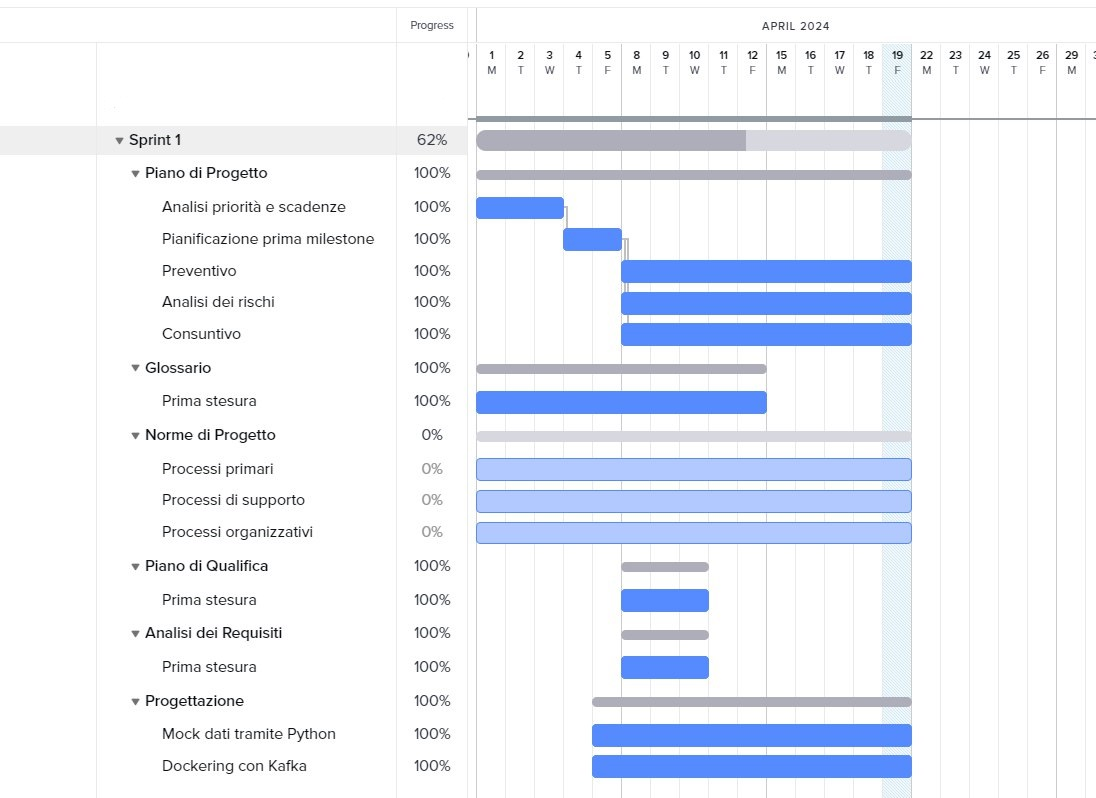
\includegraphics[width=15cm]{./images_pdp/gantt1.jpeg}
    \caption{Diagramma di Gantt rappresentativo del primo periodo.}
    \label{figure:Diagramma di Gantt rappresentativo del primo periodo}
\end{figure}
\clearpage
\newpage
\subsection{Secondo periodo} \label{sec:2_rtb}
\textbf{Inizio:} 2024-04-22\\
\textbf{Fine prevista:} 2024-05-03

\subsubsection{Pianificazione}
In questa fase del \glossterm{processo}, assume un'importanza fondamentale condurre un'analisi dettagliata del capitolato al fine di identificare accuratamente i casi d'uso necessari. Inoltre, al fine di evitare ambiguità e decisioni errate, si raccomanda di organizzare uno o più incontri con il \glossterm{Proponente} per condividere le idee e risolvere i dubbi emersi durante l'analisi, che sarà notevolmente più approfondita rispetto a quella svolta durante la selezione del \glossterm{capitolato}. Da questo processo di analisi, si darà inizio alla stesura dell'\textit{Analisi dei Requisiti}, un documento di vitale importanza per il progetto poiché conterrà tutti i casi d'uso individuati, nonché i requisiti obbligatori, desiderabili e opzionali.
È altresì consigliabile redigere il \textit{Piano di Qualifica} in questa fase, il quale sarà fondamentale per definire i metodi volti a garantire la \glossterm{qualità} dei processi e dei prodotti nel corso dello sviluppo. \\ Seguono le attività previste per questo secondo periodo:
\begin{itemize}
\setlength{\itemsep}{0em}
    \item Conclusione della sezione di Analisi dei Rischi nel documento \textit{Piano di Progetto};
    \item Aggiunta di nuovi termini al \textit{Glossario};
    \item Avvio della stesura delle \textit{Norme di Progetto};
    \item Arricchimento del documento \textit{Piano di Qualifica};
    \item Proseguimento della scrittura dell'\textit{Analisi dei Requisiti};
    \item Sintesi del funzionamento del generatore dati in un documento apposito;
    \item Realizzazione della persistenza dei dati e visualizzazione delle informazioni tramite \glossterm{dashboard}.
\end{itemize}

\subsubsection{Rischi attesi}
In questo secondo periodo prevediamo che si possano manifestare le seguenti problematiche: 
\begin{itemize}
\setlength{\itemsep}{0em}
\item \textbf{RT-1}: Inesperienza;
\item \textbf{RT-2}: Produzione di codice incomprensibile;
\item \textbf{RC-4}: Confusione nella rotazione dei ruoli;
\item \textbf{RP-1}: Stima errata delle tempistiche di progetto;
\item \textbf{RP-2}: Stima errata dei costi di progetto;
\item \textbf{RP-3}: Stima errata del tempo di completamento di un'attività.
\end{itemize}
Alcuni dei rischi identificati sono attribuibili alla limitata esperienza del gruppo, come evidenziato nei verbali, e alla persistenza di lievi difficoltà nello svolgimento delle attività, tra cui la suddivisione dei compiti assegnati. Inoltre, in concomitanza dell'inizio di questo \glossterm{Sprint} avverrà la prima rotazione dei ruoli ricoperti da ciascun membro, da cui deriva l'aggiunta di \textbf{RC-4} ai rischi previsti. Durante lo Sprint precedente il gruppo ha dimostrato una notevole coesione ed una buona capacità di gestire efficacemente eventuali divergenze di opinioni, pertanto non si è ritenuto necessario mantenere \textbf{RC-3: Conflitti interni} nella lista dei rischi attesi. Infine, è stato aggiunto \textbf{RT-2} per via dell'inizio dello sviluppo del codice per il \glossterm{Proof of Concept} (PoC).
\clearpage
\subsubsection{\glossterm{Preventivo}}
\subsubsubsection{Preventivo orario}
\begin{table}[ht!]
	\centering
	\begin{tabular}{p{4cm} p{1cm} p{1cm} p{1cm} p{1cm} p{1cm} p{1cm} p{3cm}}
        \toprule
        \textbf{Membro} & \multicolumn{6}{c}{\textbf{Ruoli}} & \textbf{Totale (persona)}\\
		& \textbf{AM} & \textbf{RE} & \textbf{PT} & \textbf{AN} & \textbf{PR} & \textbf{VE}\\
		\midrule
        Linda Barbiero          & 3     & -     & 2     & -     & 4     & 3     & 12 \\
        Guglielmo Barison       & 1     & -     & 2,5     & -     & 2   & 1     & 6,5\\
        Pietro Busato           & 1     & -     & 2,5     & -     & 2   & 1     & 6,5 \\
        Davide Donanzan         & 1     & -     & 2     & 2     & 3     & 1   & 9 \\
        Oscar Konieczny         & -     & -     & 2     & -     & 6     & 1     & 9 \\
        Veronica Tecchiati      & 2     & 3     & -     & 2     & 0     & 1     & 8 \\
        \bottomrule
        \textbf{Totale (ruolo)} & 8     & 3     & 11     & 4   & 17     & 8   & 51 \\
	\end{tabular}
	\caption{Distribuzione delle ore del secondo Sprint secondo ruolo e membro.}
	\label{table:Distribuzione delle ore del secondo Sprint secondo ruolo e membro}
\end{table}
\begin{figure}[ht!]
    \centering
    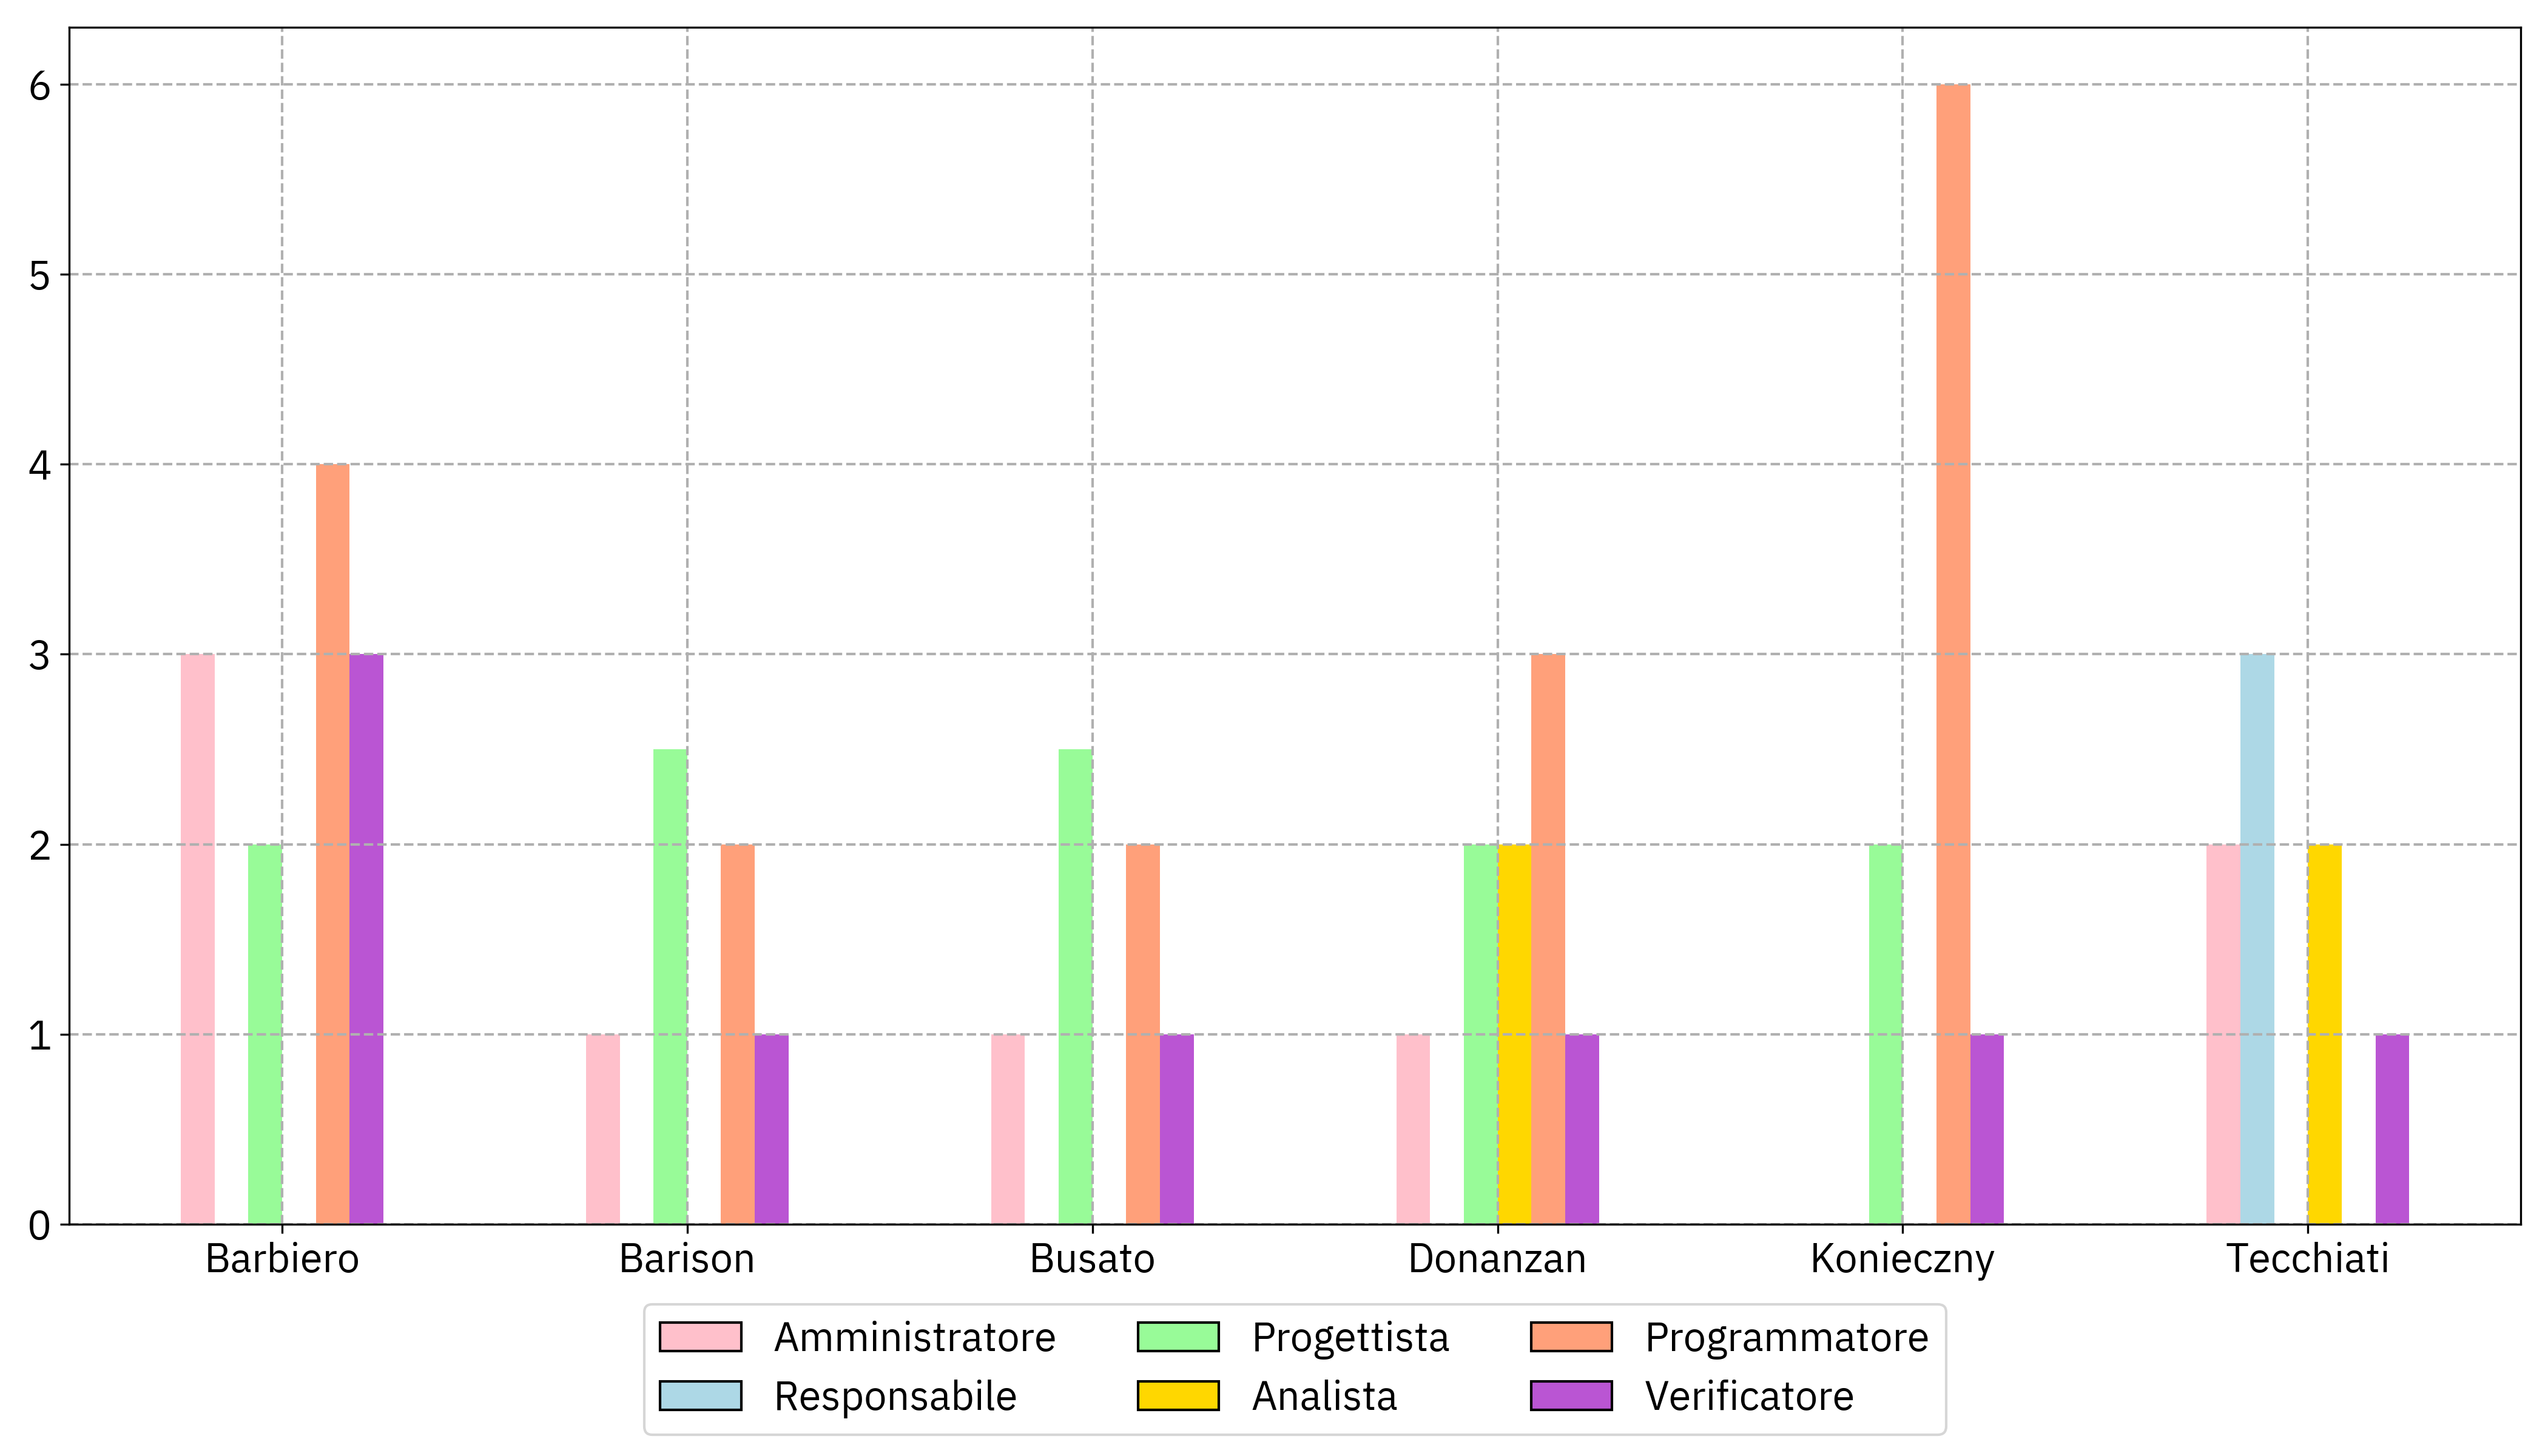
\includegraphics[width=15cm]{./images_pdp/istogramma_periodo_2.png}
    \caption{Visualizzazione dell’impegno temporale di ciascun membro nei rispettivi ruoli assegnati
    nel secondo Sprint.}
    \label{figure:Visualizzazione dell’impegno temporale di ciascun membro nei rispettivi ruoli
    assegnati nel secondo Sprint}
\end{figure}
\subsubsubsection{Preventivo economico}
\begin{table}[ht!]
	\centering
	\begin{tabular}{p{4cm} p{1cm} p{2cm}}
        \toprule
        \textbf{Ruolo} & \textbf{Ore} & \textbf{Costo (€)} \\
        \midrule
        Amministratore & 8 & 240 \\
        Responsabile & 3 & 60 \\
        Progettista & 11 & 275 \\
        Analista & 4 & 100 \\
        Programmatore & 17 & 255 \\
        Verificatore & 8 & 120 \\
        \bottomrule
        \textbf{Totale} & 51 & 1050
    \end{tabular}
    \caption{\glossterm{Preventivo} dei costi del secondo Sprint secondo ruolo.}
	\label{table:Preventivo dei costi del secondo Sprint secondo ruolo}
\end{table}
\subsubsection{\glossterm{Consuntivo}}
\subsubsubsection{Consuntivo orario}
\begin{table}[ht!]
	\centering
	\begin{tabular}{p{3cm} p{1.4cm} p{1.6cm} p{1.5cm} p{1.5cm} p{1.5cm} p{1.5cm} p{1cm}}
		\toprule
        \textbf{Membro} & \multicolumn{5}{c}{\textbf{Ruoli}} & \multicolumn{2}{r}{\textbf{Totale (pers.)}}\\
		& \textbf{AM} & \textbf{RE} & \textbf{PT} & \textbf{AN} & \textbf{PR} & \textbf{VE}\\
		\midrule
        Linda Barbiero          & 4 \textcolor{red}{(+1)} & - & 1 \textcolor{teal}{(-1)}  & - & 2
        \textcolor{teal}{(-2)} & 3 & 10 \\
        Guglielmo Barison       & - & - & 2,5 & -     & 3 \textcolor{red}{(+1)}  & 1     & 6,5\\
        Pietro Busato           & 1     & -     & 2,5     & -     & 3 \textcolor{red}{(+1)}  & 1     & 7,5 \\
        Davide Donanzan         & - \textcolor{teal}{(-1)}    & -     & 2     & 2     & 2
        \textcolor{teal}{(-1)}     & 1     & 7 \\
        Oscar Konieczny         & -   & -     & 2     & -     & 6     & 1     & 9 \\
        Veronica Tecchiati      & 2   & 3,5 \textcolor{red}{(+0,5)}     & -     & 2     & -     & 1     & 8,5 \\
        \bottomrule
        \textbf{Totale (ruolo)} & 7    & 3,5     & 10     & 4   & 16     & 8   & 48,5 \\
	\end{tabular}
	\caption{Distribuzione delle ore del secondo Sprint secondo ruolo e membro.}
	\label{table:Distribuzione delle ore consuntive del secondo Sprint secondo ruolo e membro}
\end{table}
\begin{table}[ht!]
	\centering
	\begin{tabular}{p{4cm} p{1cm} p{1cm} p{1cm} p{1cm} p{1cm} p{1cm} p{3cm}}
		\toprule
        \textbf{Membro} & \multicolumn{6}{c}{\textbf{Ruoli}} & \textbf{Totale (persona)}\\
		& \textbf{AM} & \textbf{RE} & \textbf{PT} & \textbf{AN} & \textbf{PR} & \textbf{VE}\\
		\midrule
        Linda Barbiero          & 3     & 5     & 19     & 11   & 22     & 19,5   & 79,5 \\
        Guglielmo Barison       & 4     & 9     & 16,5     & 11   & 18,5   & 21     & 80\\
        Pietro Busato           & 5     & 8     & 16,5     & 11   & 17,5   & 21     & 79\\
        Davide Donanzan         & 6     & 8     & 18     & 7    & 21     & 20     & 80\\
        Oscar Konieczny         & 4,5   & 7     & 18     & 11   & 18     & 22     & 80,5\\
        Veronica Tecchiati      & 2,5   & 4,5     & 20     & 4    & 25     & 21     & 77\\
        \bottomrule
        \textbf{Totale (ruolo)} & 25    & 41,5    & 108    & 55   & 122     & 124,5 & 476 \\
	\end{tabular}
	\caption{Ore rimaste dopo il secondo Sprint secondo ruolo e membro.}
	\label{table:Ore rimaste dopo il secondo Sprint secondo ruolo e membro}
\end{table}
\subsubsubsection{Consuntivo economico}
\begin{table}[ht!]
	\centering
	\begin{tabular}{p{4cm} p{2cm} p{2cm}}
        \toprule
        \textbf{Ruolo} & \textbf{Ore} & \textbf{Costo (€)} \\
        \midrule
        Amministratore & 7 \textcolor{teal}{(-1)} & 210 \textcolor{teal}{(-30)}\\
        Responsabile & 3,5 \textcolor{red}{(+0,5)} & 70 \textcolor{red}{(+10)} \\
        Progettista & 10 \textcolor{teal}{(-1)} & 250 \textcolor{teal}{(-25)} \\
        Analista & 4 & 100 \\
        Programmatore & 16 \textcolor{teal}{(-1)} & 240 \textcolor{teal}{(-15)} \\
        Verificatore & 8 & 120 \\
        \bottomrule
        \textbf{Totale} & 48,5 \textcolor{teal}{(-2,5)} & 990 \textcolor{teal}{(-60)}
    \end{tabular}
    \caption{\glossterm{Preventivo} a finire dei costi del secondo Sprint secondo ruolo.}
	\label{table:Preventivo a finire dei costi del secondo Sprint secondo ruolo}
\end{table}
\subsubsubsection{Rischi occorsi, impatto e loro mitigazione}
Durante questo periodo sono emerse alcune delle complicazioni previste, in particolar modo quelle riguardanti la pianificazione. Alcune attività hanno subito dei lievi ritardi, il che comporta la necessità di proseguirne lo svolgimento durante lo Sprint successivo. Inoltre, al termine dello Sprint è stata rilevata una discrepanza tra i costi preventivati e quelli effettivi, seppure la differenza sia minima. Nonostante ciò, l'impatto complessivo delle suddette problematiche sullo svolgimento del progetto non è da considerarsi allarmante.
\subsubsection{Retrospettiva}
Come anticipato nella sezione precedente, il gruppo ha riscontrato alcune difficoltà legate alla pianificazione. In particolare, l'identificazione e la suddivisione dei nuovi incarichi è avvenuta qualche giorno dopo la data di inizio dello Sprint, pertanto nei primi giorni il team si è dedicato solamente alla prosecuzione delle attività già avviate nel precedente periodo. In seguito ad un confronto con il \glossterm{Committente}, il gruppo ha deciso di introdurre un incontro di Sprint Planning subito dopo lo svolgimento del \glossterm{SAL} con la \glossterm{Proponente}, così da delineare immediatamente l'organizzazione del periodo. Nonostante questo iniziale scoglio il gruppo è riuscito comunque a soddisfare le aspettative della Proponente in merito alla scrittura del codice e ad avanzare con la stesura della documentazione. \\
Al termine del secondo periodo è emerso un lieve divario tra i costi previsti e quelli effettivi.
Infatti, il consuntivo riporta una spesa totale di 990\;\texteuro\ anziché i 1\,.050\;\texteuro\ calcolati
nel preventivo. La differenza di 60\;\texteuro\ è dovuta allo svolgimento di un minor quantitativo di
ore da Amministratore, Progettista e Programmatore rispetto alle stime, nonostante il leggero
surplus per il ruolo da Responsabile. Il budget rimanente ammonta dunque a 9\,.352,5\;\texteuro. 
\begin{figure}[h]
    \centering
    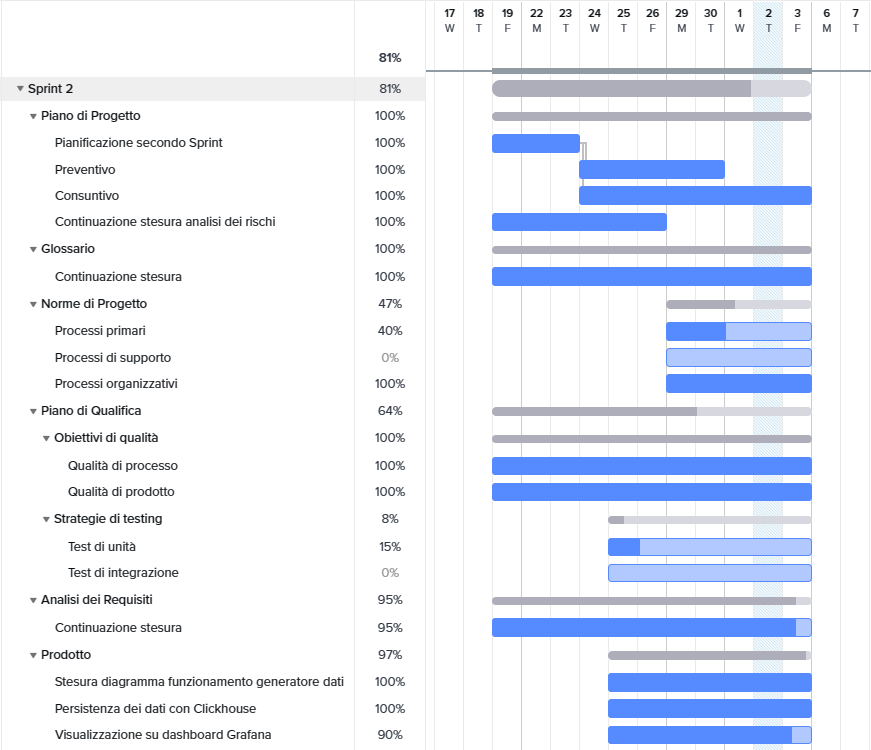
\includegraphics[width=13cm]{./images_pdp/gantt2.png}
    \caption{Diagramma di Gantt rappresentativo del secondo periodo.}
    \label{figure:Diagramma di Gantt rappresentativo del secondo periodo}
\end{figure}
\newpage
\clearpage
\subsection{Terzo periodo} \label{sec:3_rtb}
\textbf{Inizio:} 2024-05-06\\
\textbf{Fine prevista:} 2024-05-17
\subsubsection{Pianificazione}
Con il consolidamento dell'\textit{Analisi dei Requisiti}, diventa fondamentale approfondire gli
strumenti necessari per l'implementazione finale del prodotto. Il \glossterm{Proof of Concept} (PoC) ha
raggiunto un buon grado di avanzamento, anche grazie all'inclusione della componente di
visualizzazione nello \glossterm{Sprint} Backlog, originariamente pianificata per questo periodo.
Prevediamo di completarlo entro il periodo attuale, consentendo così ai programmatori di terminare
il lavoro e successivamente a tutti i membri di dedicarsi al completamento della documentazione, in
vista della prima revisione del progetto. Questo permetterà di realizzare una versione semplificata
del prodotto finale, volta a fornire indicazioni sulla validità della direzione intrapresa e a
dimostrare al \glossterm{Committente} la correttezza dell'approccio di sviluppo.\\
Considerando il progresso fatto nelle \textit{Norme di Progetto} durante il primo e il secondo
periodo, ora l'attenzione sarà principalmente rivolta a quest'ultime, la cui struttura di base è
stata precedentemente definita. L'obiettivo sarà quello di consolidare ulteriormente il documento,
riflettendo sui dettagli emersi e aggiungendo nuove informazioni.\\
Le attivit\`{a} previste durante questo periodo sono quindi le seguenti:
\begin{itemize}
\setlength{\itemsep}{0em}
    \item Arricchimento del documento \textit{Norme di progetto} precedentemente avviato;
    \item Integrazione della terminologia mancante nel documento \textit{Glossario};
    \item Consolidamento del documento \textit{Analisi dei Requisiti};
    \item Ampliamento del \textit{Piano di Qualifica};
    \item Consolidamento del PoC (\glossterm{Proof of Concept}).
\end{itemize}
\subsubsection{Rischi attesi}
I rischi che ci aspettiamo di correre in questo periodo sono i seguenti: 
\begin{itemize}
\setlength{\itemsep}{0em}
\item \textbf{RT-1:} Inesperienza;
\item \textbf{RP-1:} Stima errata delle tempistiche di progetto;
\item \textbf{RP-2:} Stima errata dei costi di progetto;
\item \textbf{RP-5:} Impegni personali ed accademici;
\end{itemize}
Il consistente carico di lavoro di questo periodo richiederà inevitabilmente più tempo ad ogni membro del gruppo. I rischi identificati sono tecnici ed organizzativi: questi potrebbero causare rallentamenti generali e ritardi.
\clearpage
\subsubsection{\glossterm{Preventivo}}
\subsubsubsection{Preventivo orario}
\begin{table}[ht!]
    \centering
    \begin{tabular}{p{4cm} p{1cm} p{1cm} p{1cm} p{1cm} p{1cm} p{1cm} p{3cm}}
        \toprule
        \textbf{Membro} & \multicolumn{6}{c}{\textbf{Ruoli}} & \textbf{Totale (persona)}\\
		& \textbf{AM} & \textbf{RE} & \textbf{PT} & \textbf{AN} & \textbf{PR} & \textbf{VE}\\
		\midrule
        Linda Barbiero       & -   & -   & 2   & -   & 5   & 4   & 11 \\
        Guglielmo Barison    & 2   & 4   & -   & -   & 1   & 2,5 & 9,5 \\
        Pietro Busato        & 4   & -   & -   & 4   & -   & 2   & 10 \\
        Davide Donanzan      & -   & -   & 2   & -   & 5   & 4   & 11 \\
        Oscar Konieczny      & 4   & -   & -   & 4   & -   & 3   & 11 \\
        Veronica Tecchiati   & -   & -   & 2   & -   & 5   & 5   & 12 \\
        \bottomrule
        \textbf{Totali (ruolo)} & 10 & 4 & 6 & 8 & 16 & 20,5 & 64,5 \\
    \end{tabular}
    \caption{Distribuzione delle ore del terzo Sprint secondo ruolo e membro.}
    \label{table:Distribuzione delle ore del terzo Sprint secondo ruolo e membro}
\end{table}
\begin{figure}[ht!]
    \centering
    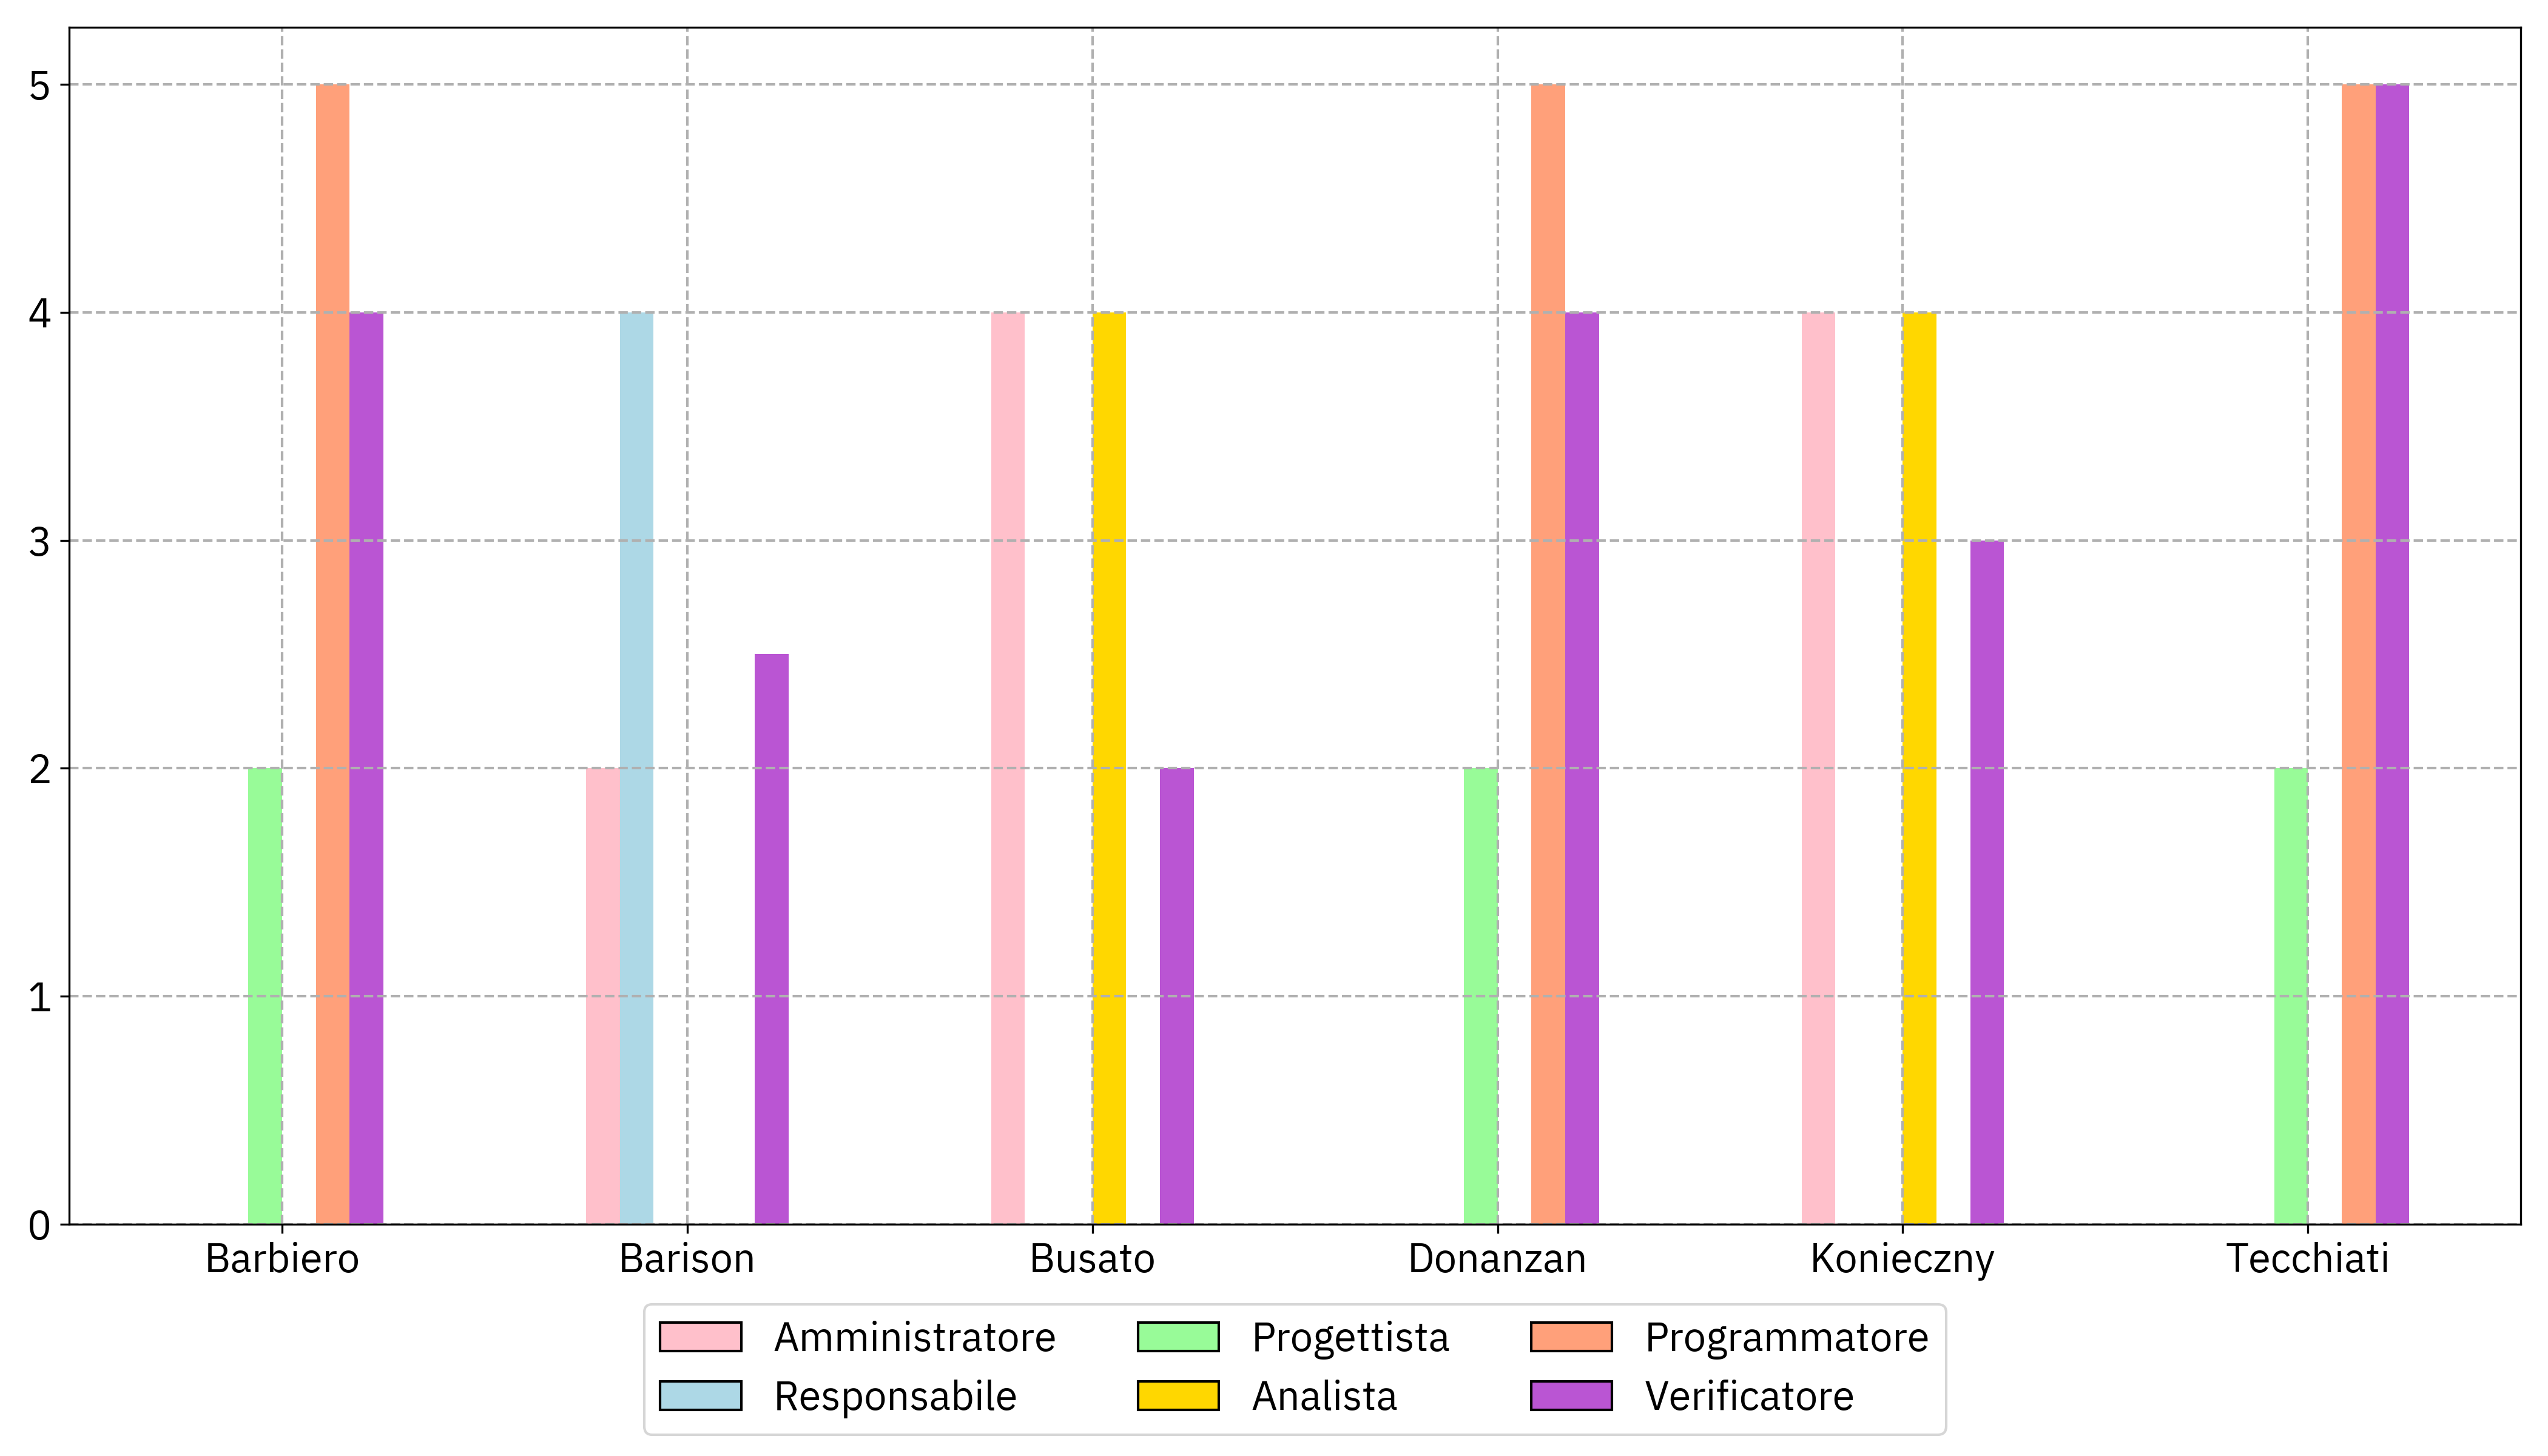
\includegraphics[width=15cm]{./images_pdp/istogramma_periodo_3.png}
    \caption{Visualizzazione dell’impegno temporale di ciascun membro nei rispettivi ruoli assegnati
    nel terzo Sprint.}
    \label{figure:Visualizzazione dell’impegno temporale di ciascun membro nei rispettivi ruoli
    assegnati nel terzo Sprint}
\end{figure}
\subsubsubsection{Preventivo economico}
\begin{table}[ht!]
	\centering
	\begin{tabular}{p{4cm} p{1cm} p{2cm}}
        \toprule
        \textbf{Ruolo} & \textbf{Ore} & \textbf{Costo (€)} \\
        \midrule
        Amministratore & 10 & 300 \\
        Responsabile & 4 & 80 \\
        Progettista & 6 & 150 \\
        Analista & 8 & 200 \\
        Programmatore & 16 & 240 \\
        Verificatore & 20.5 & 307,5 \\
        \bottomrule
        \textbf{Totale} & 64,5 & 1277,5
    \end{tabular}
    \caption{\glossterm{Preventivo} dei costi del terzo Sprint secondo ruolo.}
	\label{table:Preventivo dei costi del terzo Sprint secondo ruolo}
\end{table}
\subsubsection{\glossterm{Consuntivo}}
\subsubsubsection{Consuntivo orario}
\begin{table}[ht!]
	\centering
	\begin{tabular}{p{3cm} p{1.4cm} p{1.6cm} p{1.7cm} p{1.4cm} p{1.4cm} p{1.5cm} p{2cm}}
		\toprule
        \textbf{Membro} & \multicolumn{5}{c}{\textbf{Ruolo}} & \multicolumn{2}{r}{\textbf{Totale (persona)}}\\
		& \textbf{AM} & \textbf{RE} & \textbf{PT} & \textbf{AN} & \textbf{PR} & \textbf{VE}\\
		\midrule
        Linda Barbiero     & - & - & 2 & -   & 5 & 4 & 11 \\
        Gugliemo Barison   & 2 & 4 & - & -   & 1 & 2,5 & 9,5 \\
        Pietro Busato      & 3 \textcolor{teal}{(-1)} & - & - & 3.5
        \textcolor{red}{(-1.5)} & - & 1 \textcolor{teal}{(-1)} & 7,5 \\
        Davide Donanzan    & - & - & 2 & -   & 5 & 4 & 11 \\
        Oscar Konieczny    & 4 & - & - & 4   & - & 3 & 11 \\
        Veronica Tecchiati & 1 \textcolor{red}{(+1)} & -  & 2 & -   & 3 \textcolor{teal}{(-2)} & 4
        \textcolor{teal}{(-1)}  & 10 \\
        \midrule
        \textbf{Totale (ruolo)} & 10 & 4 & 6 & 7,5 & 14 & 18,5 & 60 \\
		\bottomrule
	\end{tabular}
	\caption{Distribuzione delle ore del terzo Sprint secondo ruolo e membro.}
	\label{table:Distribuzione delle ore del terzo Sprint secondo ruolo e membr}
\end{table}
\begin{table}[ht!]
	\centering
	\begin{tabular}{p{3cm} p{1.4cm} p{1.6cm} p{1.5cm} p{1.5cm} p{1.5cm} p{1.5cm} p{2cm}}
		\toprule
        \textbf{Membro} & \multicolumn{5}{c}{\textbf{Ruolo}} & \multicolumn{2}{r}{\textbf{Totale (persona)}}\\
		& \textbf{AM} & \textbf{RE} & \textbf{PT} & \textbf{AN} & \textbf{PR} & \textbf{VE}\\
		\midrule
        Linda Barbiero     & 3 & 5 & 17 & 11   & 17 & 15,5 & 68,5 \\
        Gugliemo Barison   & 2 & 5 & 16,5 & 11   & 17,5 & 18,5 & 70,5 \\
        Pietro Busato      & 2 & 8 & 16,5 & 7,5 & 17,5 & 20 & 71,5 \\
        Davide Donanzan    & 6 & 8 & 16 & 7   & 16 & 16 & 69 \\
        Oscar Konieczny    & 0,5 & 7 & 18 & 7   & 18 & 19 & 69,5 \\
        Veronica Tecchiati & 1,5 & 4,5 & 18 & 4   & 22 & 17 & 67 \\
        \midrule
        \textbf{Totale (ruolo)} & 15 & 37,5 & 102 & 47,5 & 108 & 106 & 416 \\
		\bottomrule
	\end{tabular}
	\caption{Ore rimaste dopo il terzo Sprint secondo ruolo e membro.}
	\label{table:Ore rimaste dopo il terzo Sprint secondo ruolo e membro.}
\end{table}
\subsubsubsection{Consuntivo economico}
\begin{table}[ht!]
    \centering
    \begin{tabular}{p{4cm} p{1.8cm} p{2.2cm}}
        \toprule
        \textbf{Ruolo} & \textbf{Ore} & \textbf{Costo (€)} \\
        \midrule
        Amministratore & 10 & 300 \\
        Responsabile & 4  & 80 \\
        Progettista & 6  & 150 \\
        Analista & 7,5 \textcolor{teal}{(-0,5)} & 187,5 \textcolor{teal}{(-12,5)}\\
        Programmatore & 14 \textcolor{red}{(-1)} & 210 \textcolor{teal}{(-15)}\\
        Verificatore & 18,5 \textcolor{red}{(+1,5)} & 277,5 \textcolor{red}{(+30)} \\
        \bottomrule
        \textbf{Totale} & 60 & 1205
    \end{tabular}
    \caption{\glossterm{Preventivo} a finire dei costi del terzo Sprint secondo ruolo.}
    \label{table:Preventivo a finire dei costi del terzo Sprint secondo ruolo}
\end{table}

\subsubsubsection{Rischi occorsi, impatto e loro mitigazione}
\\Nel corso di questo periodo il gruppo ha scelto di svolgere numerose attivit\`{a} in un tempo limitato.
In seguito ad un controllo generale della documentazione, sono emerse diverse imprecisioni in
particolari sezioni, sottolineando come alcune attivit\`{a} non fossero state svolte in maniera
ottimale. Gli analisti si sono occupati di sistemare queste parti. I rischi preventivati hanno avuto un impatto medio sul gruppo, causando principalmente stress, tuttavia, alla fine, sono stati mitigati nel miglior modo possibile.
\subsubsection{Retrospettiva}
Il terzo periodo si è rivelato, come da aspettative, il pi\`{u} intenso dei tre. Tutto sommato, il
carico di lavoro poteva essere distribuito diversamente, magari su pi\`{u} periodi di lavoro.
All'interno del team, è stato notevolmente valutato l'impegno di alcuni membri nel dedicare
ulteriori ore per prevenire un rallentamento eccessivo nell'avanzamento globale del progetto.
Tuttavia, sarebbe auspicabile evitare tali circostanze in futuro, sebbene abbiano messo in luce la
determinazione della maggioranza del gruppo a procedere con decisione.\\
Al termine del secondo periodo è emerso un lieve divario tra i costi previsti e quelli effettivi.
Infatti, il consuntivo riporta una spesa totale di 1\,.205\;\texteuro\ anzichè i 1\,.277,5\;\texteuro\ calcolati
nel preventivo. La differenza di 72,5\;\texteuro\ è dovuta all'indisposizione fisica di uno dei membri del gruppo, impossibilitato quindi a portare a termine tutte le ore assegnategli. Il budget rimanente ammonta dunque a 8\,.147,5\;\texteuro.
\begin{figure}[h!]
    \centering
    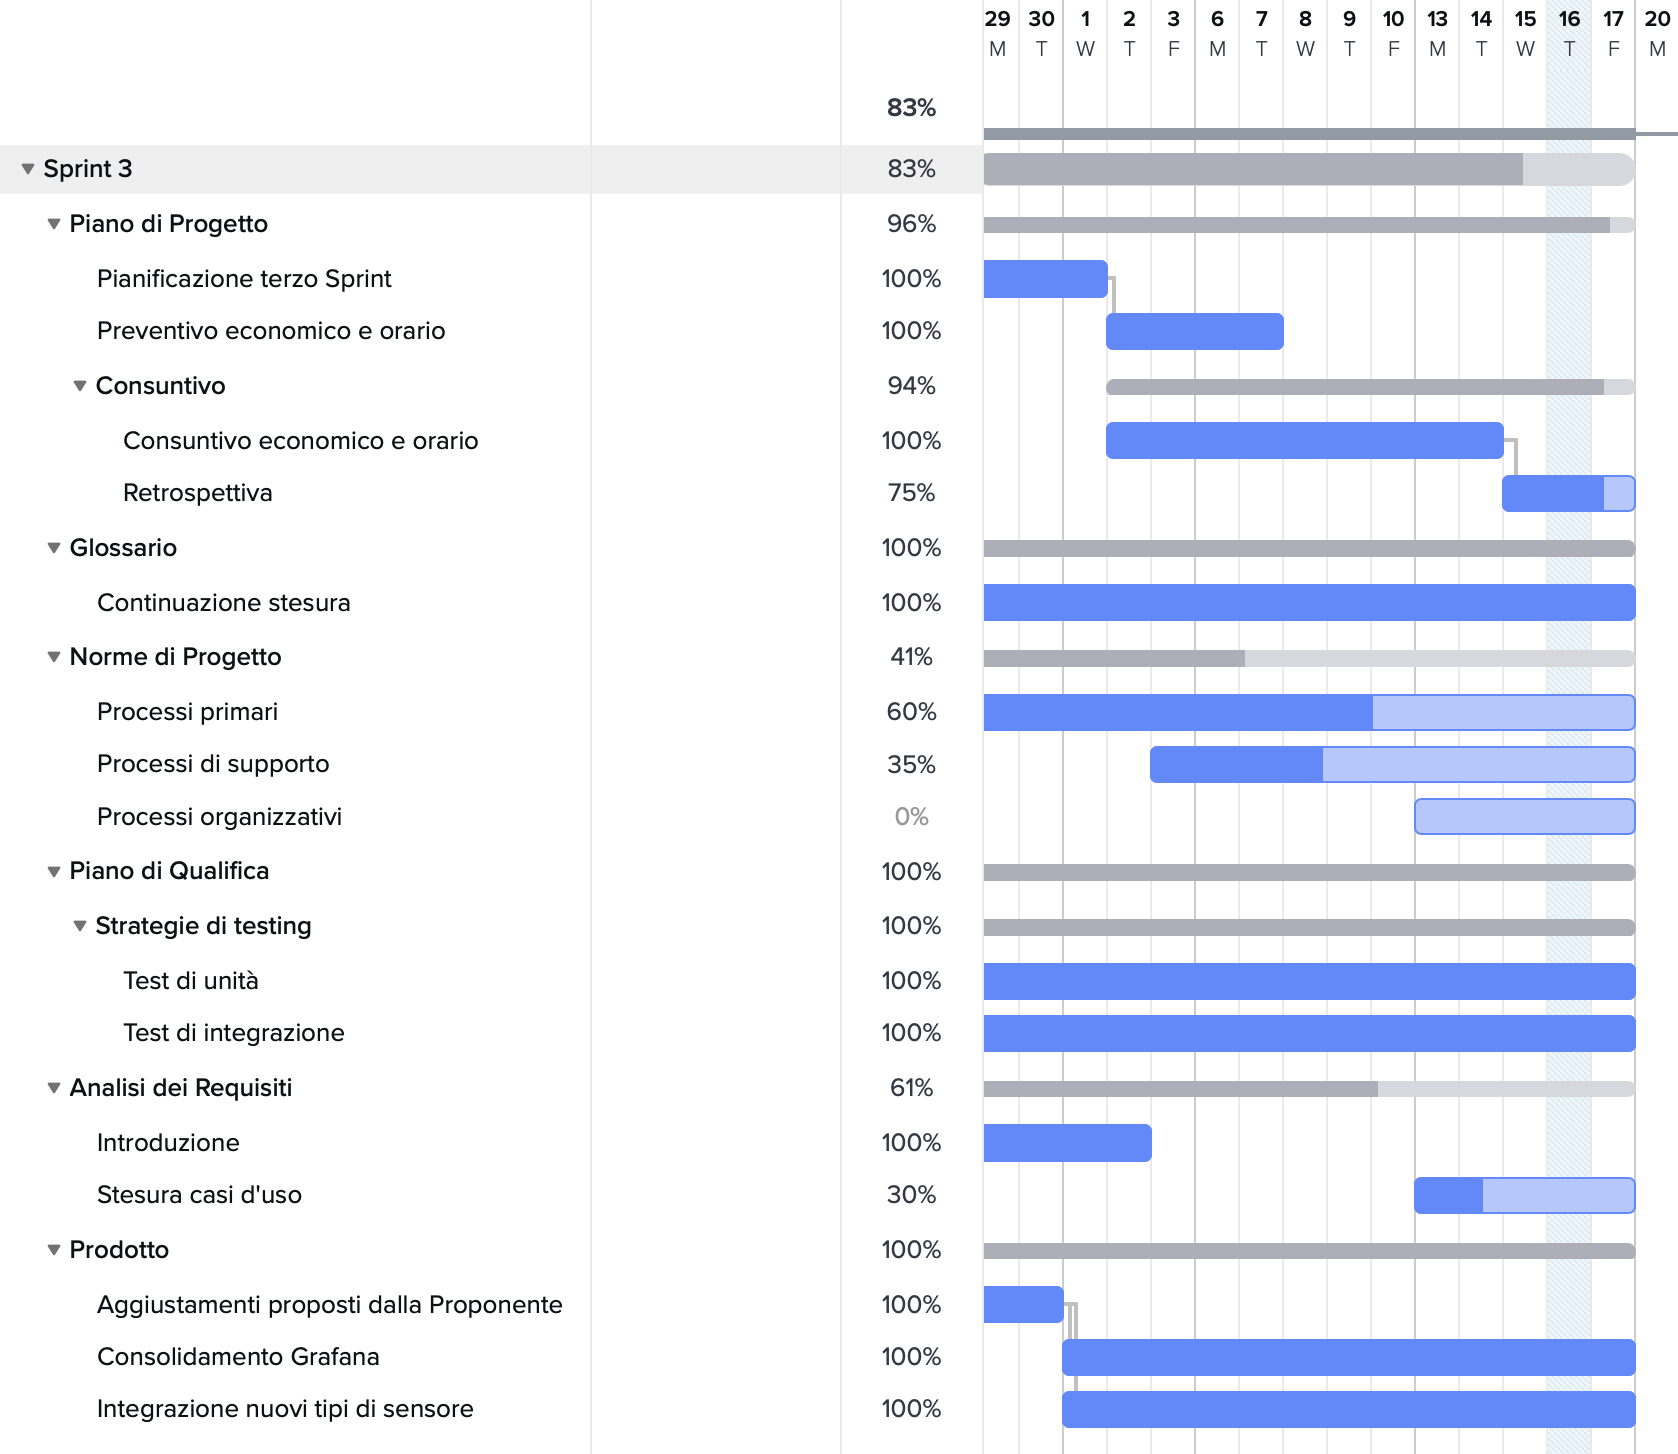
\includegraphics[width=13cm]{./images_pdp/gantt3.png}
    \caption{Diagramma di Gantt rappresentativo del terzo periodo.}
\end{figure}
\clearpage
\subsection{Quarto periodo} \label{sec:4_rtb}
\textbf{Inizio:} 2024-05-20\\
\textbf{Fine prevista:} 2024-05-31
\subsubsection{Pianificazione}
Essendo questo l'ultimo \glossterm{Sprint} di due settimane complete prima della fine della prima parte del progetto,
con conseguente presentazione del \textit{PoC}, assume primaria importanza l'ultimazione della progettazione
e implementazione di quest'ultimo, nonché una rifinitura dello stesso. Parallelamente, diventano imprescindibili
il completamento, il perfezionamento e la verifica finale di tutti documenti in vista della revisione pianificata
per l'inizio del mese di giguno. \\
Il mancato chiarimento con l'azienda proponente dell'implementazione e funzionamento di una parte del progetto,
con conseguente riscrittura e implementazione di una non indifferente porzione di codice, pone tuttavia un pericoloso
contrattempo e aggiunge una difficoltà da risolvere che va ad accatastarsi su una mole di lavoro già massicia. \\
L'avvicinamento inoltre del periodo di esami di inizio estate aggiunge infine ulteriore pressione e precarietà
alla situazione, che il team si ritiene comunque pronto ad affrontare con determinazione e grinta.\\
Le attività previste durante questo periodo sono quindi le seguenti:
\begin{itemize}
\setlength{\itemsep}{0em}
    \item Ristrutturazione e reimplementazione di parte del progetto;
    \item Rifinitura e pulitura del prodotto da presentare, ovvero il \textit{PoC};
    \item Completamento della documentazione;
    \item Rifinitura e pulitura della documentazione.
\end{itemize}
\subsubsection{Rischi attesi}
I rischi che ci aspettiamo di correre in questo periodo sono i seguenti: 
\begin{itemize}
\setlength{\itemsep}{0em}
    \item \textbf{RT-1} Inesperienza;  
    \item \textbf{RC-2} Scarsa comunicazione con la proponente;
    \item \textbf{RP-2} Stima errata dei costi di progetto;
    \item \textbf{RP-3} Stima errata del tempo di completamento di un'attività;
    \item \textbf{RP-5} Impegni personali ed accademici.
\end{itemize}
\clearpage
\subsubsection{\glossterm{Preventivo}}
\subsubsubsection{Preventivo orario}
\begin{table}[ht!]
	\centering
	\begin{tabular}{p{4cm} p{1cm} p{1cm} p{1cm} p{1cm} p{1cm} p{1cm} p{3cm}}
		\toprule
        \textbf{Membro} & \multicolumn{6}{c}{\textbf{Ruoli}} & \textbf{Totale (persona)}\\
		& \textbf{AM} & \textbf{RE} & \textbf{PT} & \textbf{AN} & \textbf{PR} & \textbf{VE}\\
		\midrule
        Linda Barbiero          & 2     & -     & 4     & 7     & 4     & 3     & 22 \\
        Guglielmo Barison       & 1     & -     & 4     & 3     & 4     & 3     & 15\\
        Pietro Busato           & 4     & 4     & 4     & 0     & 4     & 3     & 19 \\
        Davide Donanzan         & 1     & -     & 4     & 3     & 6     & 3     & 17 \\
        Oscar Konieczny         & 4     & -     & 4     & 0     & 3     & 3     & 14 \\
        Veronica Tecchiati      & 2     & -     & 4     & 5     & 1,5   & 3     & 15,5 \\
        \bottomrule
        \textbf{Totale (ruolo)} & 16    & 4     & 24    & 18    & 22,5  & 18   & 100,5 \\
	\end{tabular}
	\caption{Distribuzione delle ore del quarto Sprint secondo ruolo e membro.}
	\label{table:Distribuzione delle ore del quarto Sprint secondo ruolo e membro}
\end{table}
\begin{figure}[ht!]
    \centering
    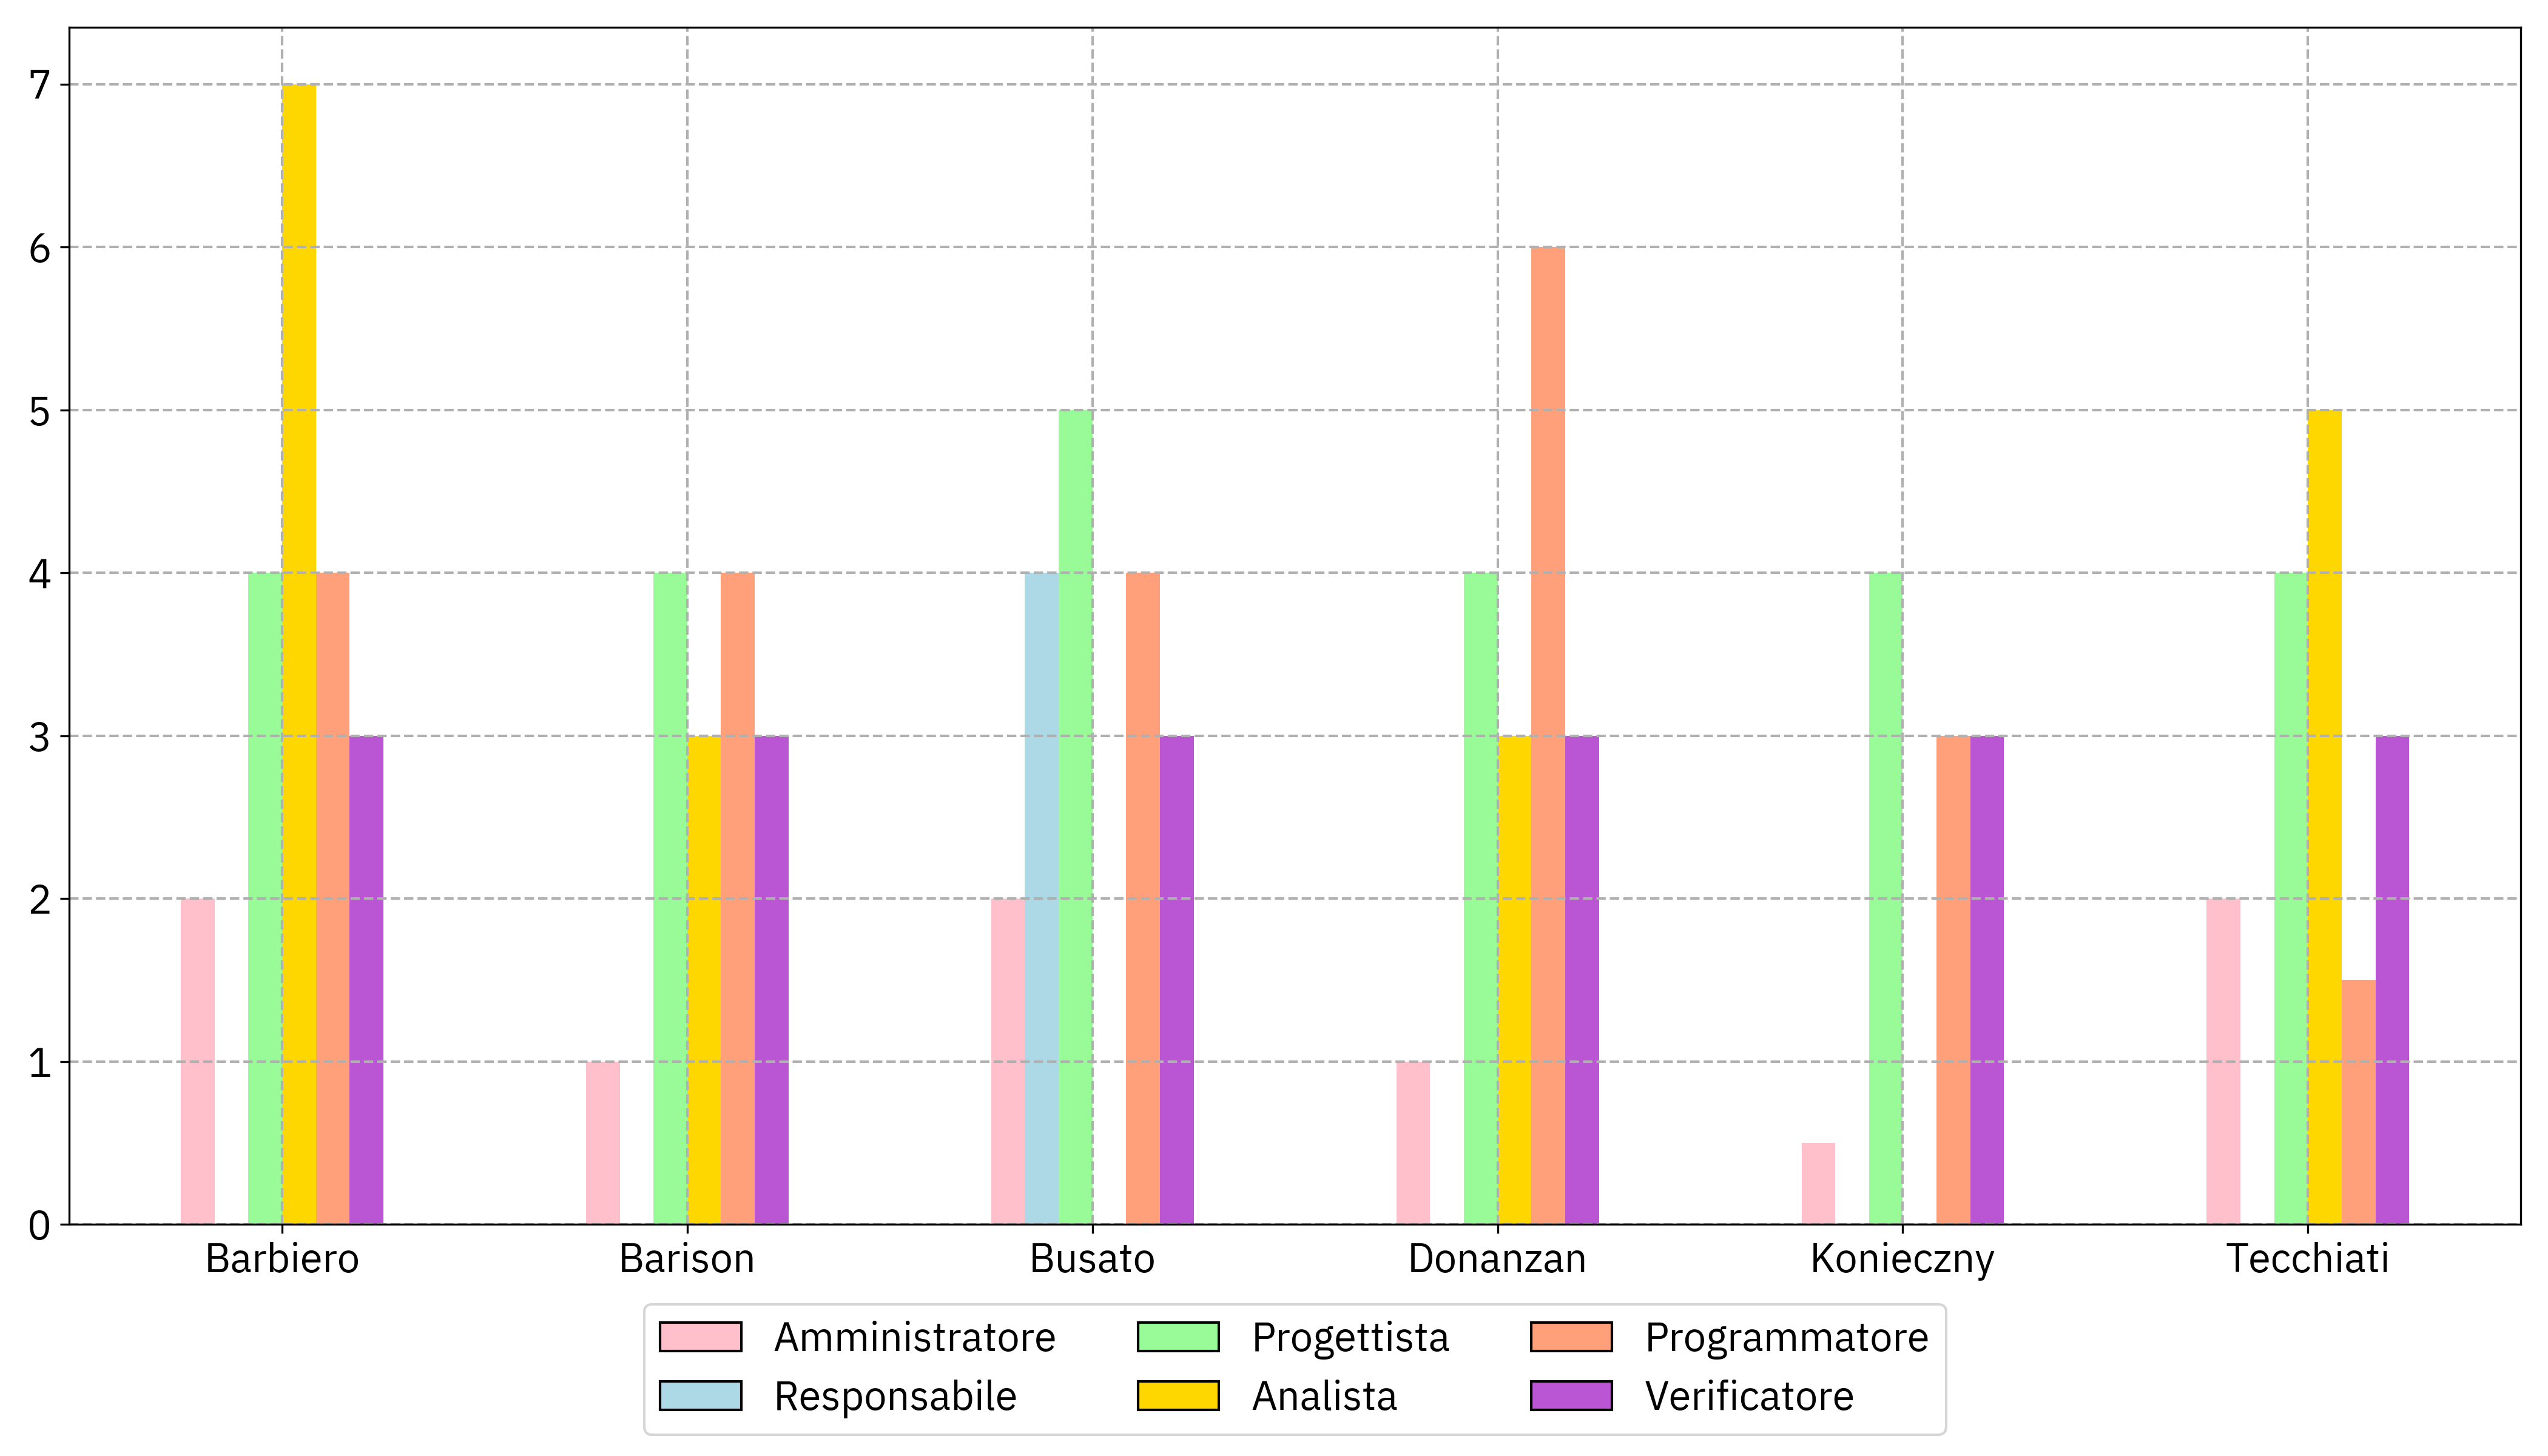
\includegraphics[width=15cm]{./images_pdp/istogramma_periodo_4.png}
    \caption{Visualizzazione dell’impegno temporale di ciascun membro nei rispettivi ruoli assegnati
    nel quarto Sprint.}
    \label{figure:Visualizzazione dell’impegno temporale di ciascun membro nei rispettivi ruoli
    assegnati nel quarto Sprint}
\end{figure}
\subsubsubsection{Preventivo economico}
\begin{table}[ht!]
	\centering
	\begin{tabular}{p{4cm} p{1cm} p{2cm}}
        \toprule
        \textbf{Ruolo} & \textbf{Ore} & \textbf{Costo (€)} \\
        \midrule
        Amministratore & 14 & 420 \\
        Responsabile & 4 & 80 \\
        Progettista & 24 & 600 \\
        Analista & 18 & 450 \\
        Programmatore & 22,5 & 337,5 \\
        Verificatore & 18 & 270 \\
        \bottomrule
        \textbf{Totale} & 100,5 & 2157,5
    \end{tabular}
    \caption{\glossterm{Preventivo} dei costi del quarto Sprint secondo ruolo.}
	\label{table:Preventivo dei costi del quarto Sprint secondo ruolo}
\end{table}
\subsubsection{\glossterm{Consuntivo}}
\subsubsubsection{Consuntivo orario}
\begin{table}[ht!]
	\centering
	\begin{tabular}{p{3cm} p{1.4cm} p{1.6cm} p{1.7cm} p{1.4cm} p{1.4cm} p{1.5cm} p{2cm}}
		\toprule
        \textbf{Membro} & \multicolumn{5}{c}{\textbf{Ruolo}} & \multicolumn{2}{r}{\textbf{Totale (persona)}}\\
		& \textbf{AM} & \textbf{RE} & \textbf{PT} & \textbf{AN} & \textbf{PR} & \textbf{VE}\\
		\midrule
        Linda Barbiero     & 1\textcolor{teal}{(-1)} & - & 3\textcolor{teal}{(-1)} & 5\textcolor{teal}{(-2)} & 5\textcolor{red}{(+1)} & 3 & 17\textcolor{teal}{(-3)} \\
        Gugliemo Barison   & 1 & - & 2\textcolor{teal}{(-2)} & 4\textcolor{red}{(+1)} & 6\textcolor{red}{(+2)} & 3,5\textcolor{red}{(+0,5)} & 16.5\textcolor{red}{(+1,5)} \\
        Pietro Busato      & 3\textcolor{teal}{(-1)} & 4 & 2\textcolor{teal}{(-2)} & 4\textcolor{red}{(+4)} & 5\textcolor{red}{(+1)} & 3 & 21\textcolor{red}{(+2)} \\
        Davide Donanzan    & 1 & - & 4 & 5\textcolor{red}{(+2)} & 7\textcolor{red}{(+1)} & 3 & 20\textcolor{red}{(+3)} \\
        Oscar Konieczny    & 3\textcolor{teal}{(-1)} & - & 3\textcolor{teal}{(-1)} & 3\textcolor{red}{(+3)} & 3.5\textcolor{red}{(+0,5)} & 4\textcolor{red}{(+1)} & 16.5\textcolor{red}{(+2,5)}\\
        Veronica Tecchiati & -\textcolor{teal}{(-2)} & - & 1\textcolor{teal}{(-3)} & 4\textcolor{teal}{(-1)} & 4\textcolor{red}{(+2,5)} & 4\textcolor{red}{(+1)} & 13\textcolor{teal}{(-2,5)} \\
        \midrule
        \textbf{Totale (ruolo)} & 9 & 4 & 15 & 25 & 30.5 & 20,5 & 104 \\
		\bottomrule
	\end{tabular}
	\caption{Distribuzione delle ore del quarto Sprint secondo ruolo e membro.}
	\label{table:Distribuzione delle ore del terzo Sprint secondo ruolo e membr}
\end{table}
\begin{table}[ht!]
	\centering
	\begin{tabular}{p{3cm} p{1.4cm} p{1.6cm} p{1.5cm} p{1.5cm} p{1.5cm} p{1.5cm} p{2cm}}
		\toprule
        \textbf{Membro} & \multicolumn{5}{c}{\textbf{Ruolo}} & \multicolumn{2}{r}{\textbf{Totale (persona)}}\\
		& \textbf{AM} & \textbf{RE} & \textbf{PT} & \textbf{AN} & \textbf{PR} & \textbf{VE}\\
		\midrule
        Linda Barbiero     & 2 & 5 & 14 & 6 & 12 & 12,5 & 68,5 \\
        Gugliemo Barison   & 1 & 5 & 14,5 & 7 & 11,5 & 15 & 54 \\
        Pietro Busato      & -1& 4 & 14,5 & 3,5 & 12,5 & 17 & 50,5 \\
        Davide Donanzan    & 5 & 8 & 12 & 2 & 9 & 13 & 49 \\
        Oscar Konieczny    & -2,5 & 7 & 15 & 4 & 14,5 & 15 & 53 \\
        Veronica Tecchiati & 1,5 & 4,5 & 17 & 0 & 18 & 13 & 54 \\
        \midrule
        \textbf{Totale (ruolo)} & 6 & 33,5 & 87 & 22,5 & 77 & 85,5 & 312 \\
		\bottomrule
	\end{tabular}
	\caption{Ore rimaste dopo il quarto Sprint secondo ruolo e membro.}
	\label{table:Ore rimaste dopo il terzo Sprint secondo ruolo e membro.}
\end{table}
\subsubsubsection{Consuntivo economico}
\begin{table}[ht!]
    \centering
    \begin{tabular}{p{4cm} p{1.8cm} p{2.2cm}}
        \toprule
        \textbf{Ruolo} & \textbf{Ore} & \textbf{Costo (€)} \\
        \midrule
        Amministratore & 9\textcolor{teal}{(-5)} & 270\textcolor{teal}{(-150)} \\
        Responsabile & 4  & 80 \\
        Progettista & 15\textcolor{teal}{(-9)}  & 375\textcolor{teal}{(-225)} \\
        Analista & 25\textcolor{red}{(+7)} & 625\textcolor{red}{(+175)} \\
        Programmatore & 30,5\textcolor{red}{(+8)} & 457,5\textcolor{red}{(+120)} \\
        Verificatore & 20,5\textcolor{red}{(+2,5)} & 307,5\textcolor{red}{(+37,5)} \\
        \bottomrule
        \textbf{Totale} & 104 & 2115
    \end{tabular}
    \caption{\glossterm{Preventivo} a finire dei costi del quarto Sprint secondo ruolo.}
    \label{table:Preventivo a finire dei costi del terzo Sprint secondo ruolo}
\end{table}
\subsubsubsection{Rischi occorsi, impatto e loro mitigazione}
Questo \glossterm{Sprint} ha visto susseguirsi numerose problematiche, principalmente riguardanti
il tempo a disposizione rispetto al carico di lavoro assegnato. Ciononostante, il team ha svolto compiti e risolto problemi con celerità
e determinazione, riuscendo a garantire il completamento degli obiettivi fissati entro il tempo
limite. Questo tuttavia ha portato il gruppo a dover redistribuire alcuni carichi di lavoro e
riassegnare parzialmente i ruoli in itinere: ne consegue che il consuntivo differisce discretamente 
dal preventivo e, sebbene da un punto di vista economico si sia riusciti a risparmiare una piccola somma
di denaro, -42,5\texteuro, il monte ore finale presenta uno scenario abbastanza diverso da quello previsto.
Un altro problema verificatosi durante lo Sprint, conseguente al ritmo accelerato di lavoro che ci si è stati trovati ad adottare, 
risiede nell'aver giocoforza rivolto minore attenzione alla cura dei dettagli di alcune parti di documentazione, che il team 
si è già riservato di ottemperare nel prossimo Sprint, della durata prevista di una singola settimana, in preparazione all'\glossterm{RTB}.
\subsubsection{Retrospettiva}
Come già precedentemente accennato, durante questo Sprint il team ha dimostrato concretamente di essere in grado di gestire in maniera adeguata
situazioni improvvise, perigliose e stringenti, con l'unica pecca di aver dovuto, in alcuni momenti, gestire i ruoli e le ore assegnate
a ciascun membro in maniera riorganizzata, sia per problemi di compatibilità con impegni personali, sia per semplificare la risoluzione 
dei vari compiti sulla base delle conoscenze pregresse e del lavoro svolto fino a quel momento da ciascuno. Al netto di essere riusciti a
mantenere pressocchè inalterato il costo finale dello Sprint e di non aver subito rallentamenti rilevanti per quanto riguarda l'avanzamento
del progetto, il gruppo dovrà tuttavia impegnarsi più a fondo per quanto riguarda la comunicazione con la \glossterm{Proponente} e il chiarimento
di eventuali dubbi sorti durante gli incontri, siano essi \glossterm{SAL} o diari di bordo: il team dovrà fare più affidamento sui canali di comunicazione
per discutere con l'azienda di probabili misinterpretazioni o mancati chiarimenti, e non esitare a chiedere consiglio ai Prof. Vardanega e Cardin
per risolvere preventivamente o evitare completamente, in futuro, situazioni simili. 
\begin{figure}[h!]
    \centering
    \includegraphics[width=13cm]{./images_pdp/gantt4.png}
    \caption{Diagramma di Gantt rappresentativo del quarto periodo.}
\end{figure}
\clearpage

\newpage
% \section\glossterm{{PB}}
% \newpage
\section{Organigramma} \label{sec:organigramma}
\subsection{Componenti}
\begin{table}[ht!]
	\centering
	\begin{tabular}{p{3cm} p{3cm}}
		\toprule
		\textbf{Nominativo} & \textbf{Matricola} \\
		\midrule
		Guglielmo Barison & 2042324 \\
		Linda Barbiero &  1220244 \\
		Pietro Busato & 2043688 \\
		Oscar Konieczny & 2042335 \\
		Davide Donanzan & 2034337 \\
		Veronica Tecchiati & 2034309 \\
		\bottomrule
	\end{tabular}
	\caption{Nominativi e matricole NaN1fy.}
	\label{table:Nominativi e matricole NaN1fy}
\end{table}

\end{document}
